\section*{Diversity Techniques in Wireless Communications}



\begin{figure}[ht]
    \centering
    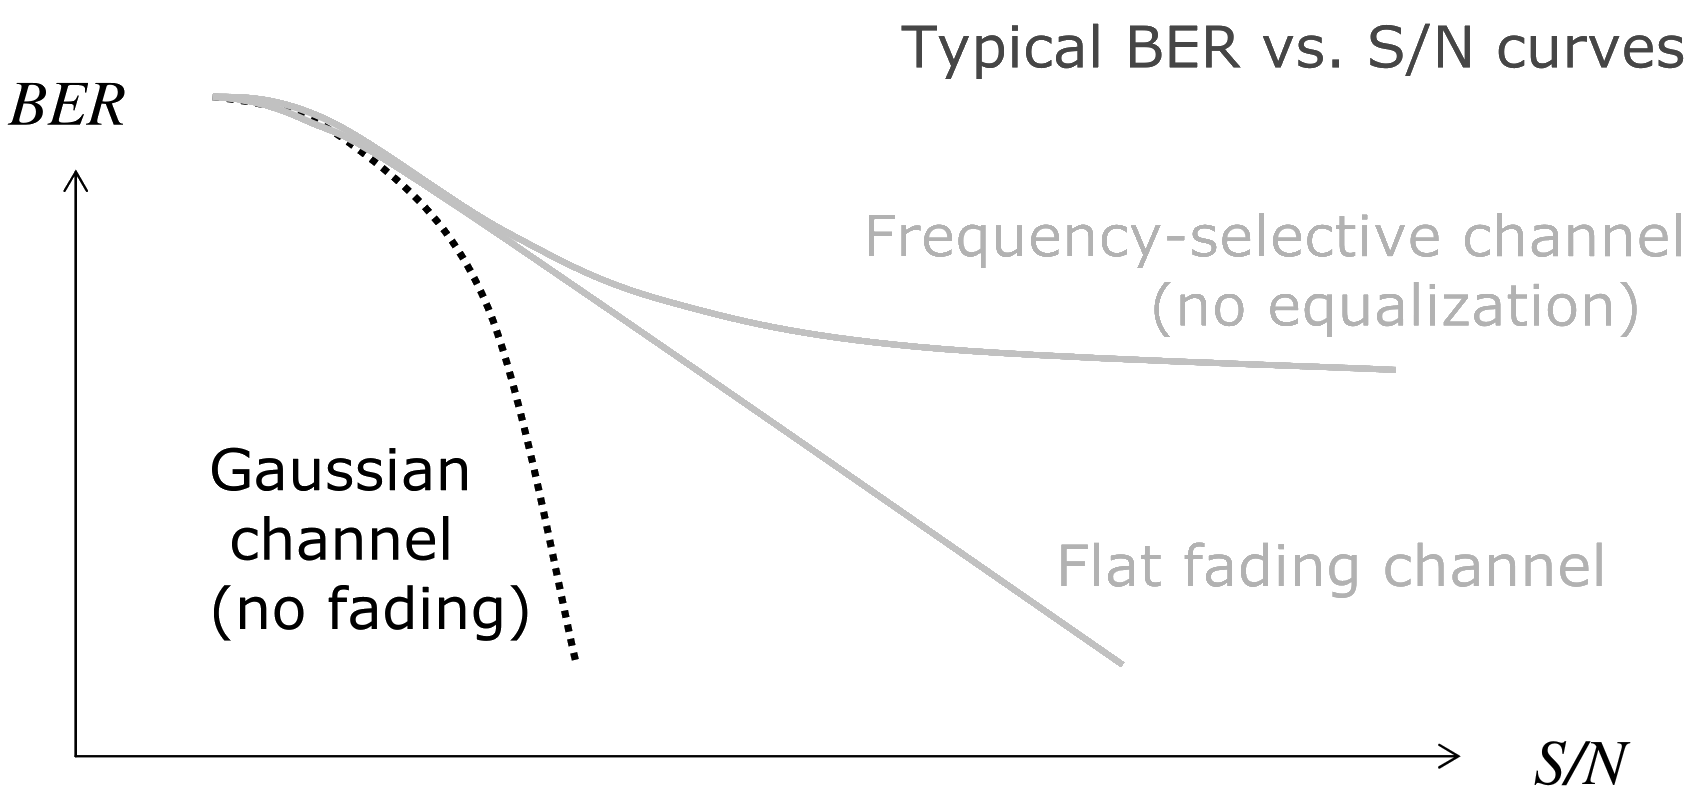
\includegraphics[width=0.675\textwidth]{imgs/bers.png}
\end{figure}


Il fading rappresenta il principale problema nelle comunicazioni radio, sebbene modulazioni come OFDM siano in grado di ridurre l'effetto del multipath fading, tuttavia lo \textbf{slow flat Rayleigh fading} non può essere contrastato nello stesso modo.

\begin{itemize}
    \item \textbf{Slow fading}: $T < T_c$ (Doppler spread)
    \item \textbf{Flat fading}: $\sigma_{\tau}<T$  (multipath time delay spread)
    \item \textbf{Rayleigh fading}: l'attenuazione delle repliche ha una distribuzione di Rayleigh.
\end{itemize}

\begin{figure}[ht]
    \centering
    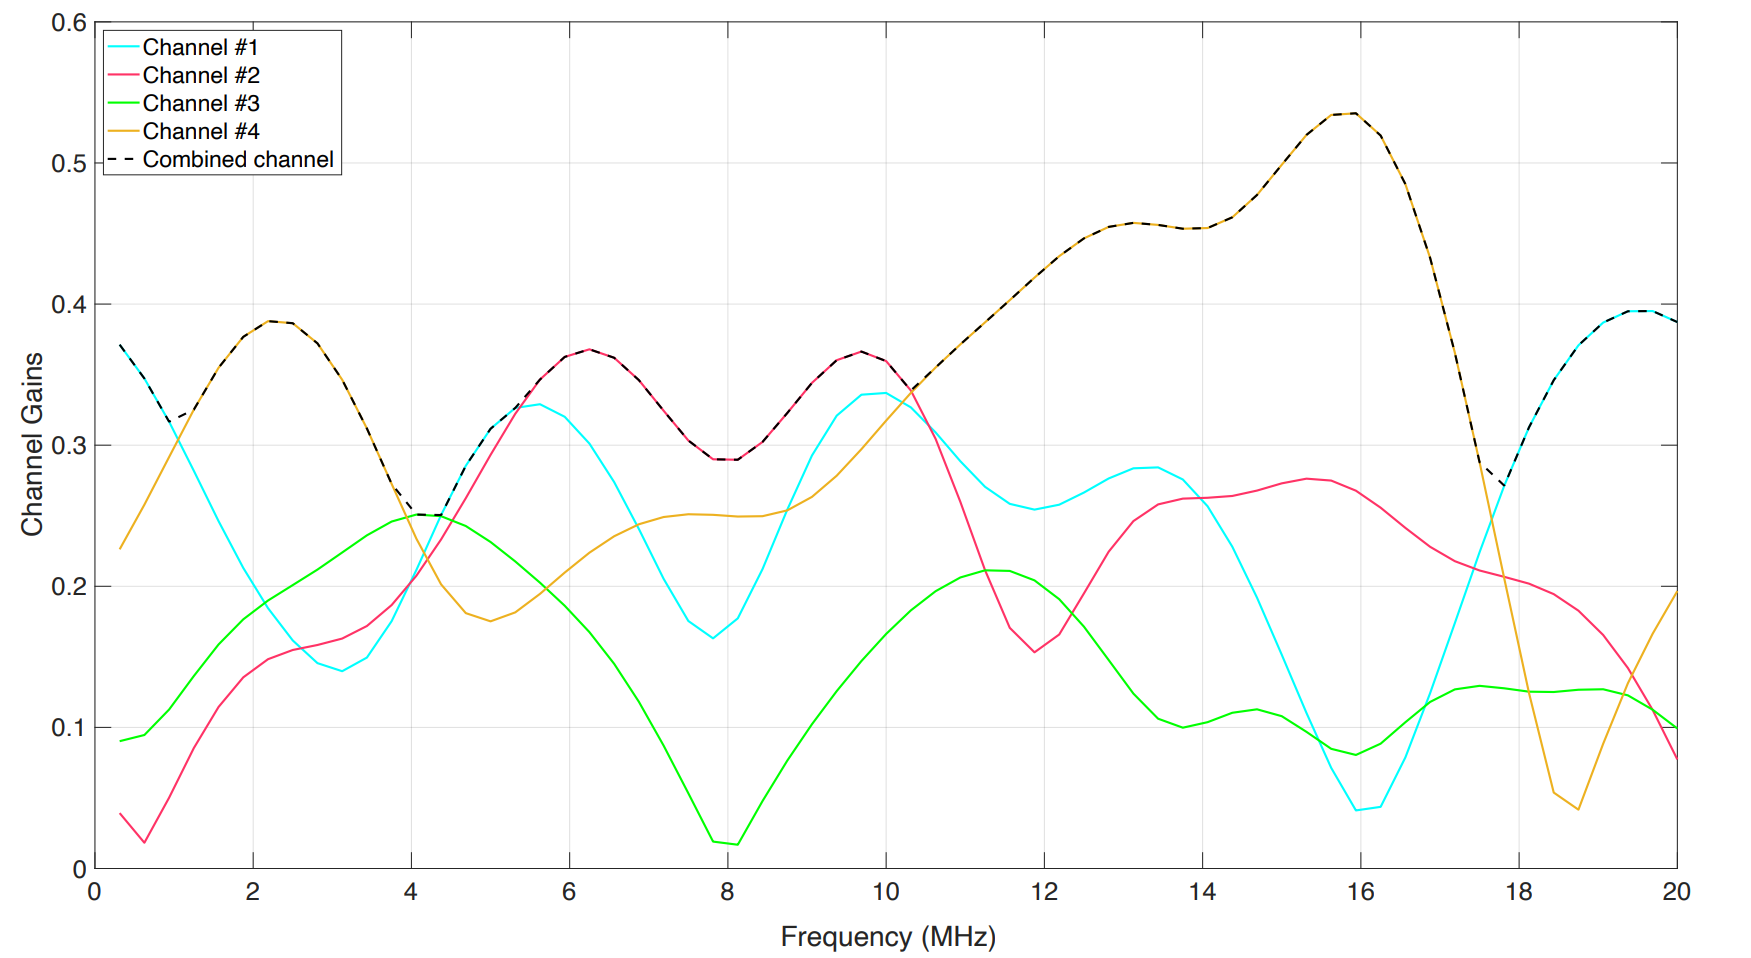
\includegraphics[width=0.675\textwidth]{imgs/diversity_graph.jpg}
\end{figure}

I metodi principali per ridurre gli effetti di un fading di tali tipologie sono le tecniche basate sulla diversità, ovvero lo sfruttamento di canali con caratteristiche differenti per trasmettere la stessa informazione, aumentando la probabilità che il ricevitore possa ricostruire correttamente il messaggio.
Le principali tecniche di diversità sono:
\begin{itemize}
    \item \textbf{Diversità temporale}: relativa al tempo di coerenza ($T_c$). Sfruttano trasmissioni in slot temporali separati utilizzando anche \textbf{coding} e \textbf{interleaving}. I canali slow fading potrebbero non garantire una diversità sufficiente. Il canale deve variare sufficientemente in maniera veloce.
    \item \textbf{Diversità in frequenza}: relativa alla banda di coerenza ($B_c$). Sfruttano tramissioni su bande differenti. I canali flat fading potrebbero non garantire una diversità sufficiente.
    \item \textbf{Diversità spaziale}: relativa alla distanza di coerenza. Sfruttano path di propagazione differenti, ad esempio antenne differenti.
\end{itemize}

\subsection*{Diversità temporale}
\paragraph*{Coding}
Il channel coding consiste nell'introdurre dei bit ridondanti insieme a quelli trasmessi per rilevare eventuali errori al ricevitore e migliorare la probabilità di errore sul bit. 
La ridondanza è misurata come:
\[
    R = \frac{k}{n} < 1, \quad \begin{cases}
        k \text{ bit contenenti informazione} \\
        n \text{ bit in uscita dall'codificatore, contenenti informazione più ridondanza} \\
        n - k \text{ bit di ridondanza}
    \end{cases}
\]

Le operazioni effettuate sfruttano le proprietà matematiche del Galois Field GF(2), su cui sono definite somma (xor) e moltiplicazione (and) per due elementi $\{0, 1\}$.

\begin{figure}[ht]
    \centering
    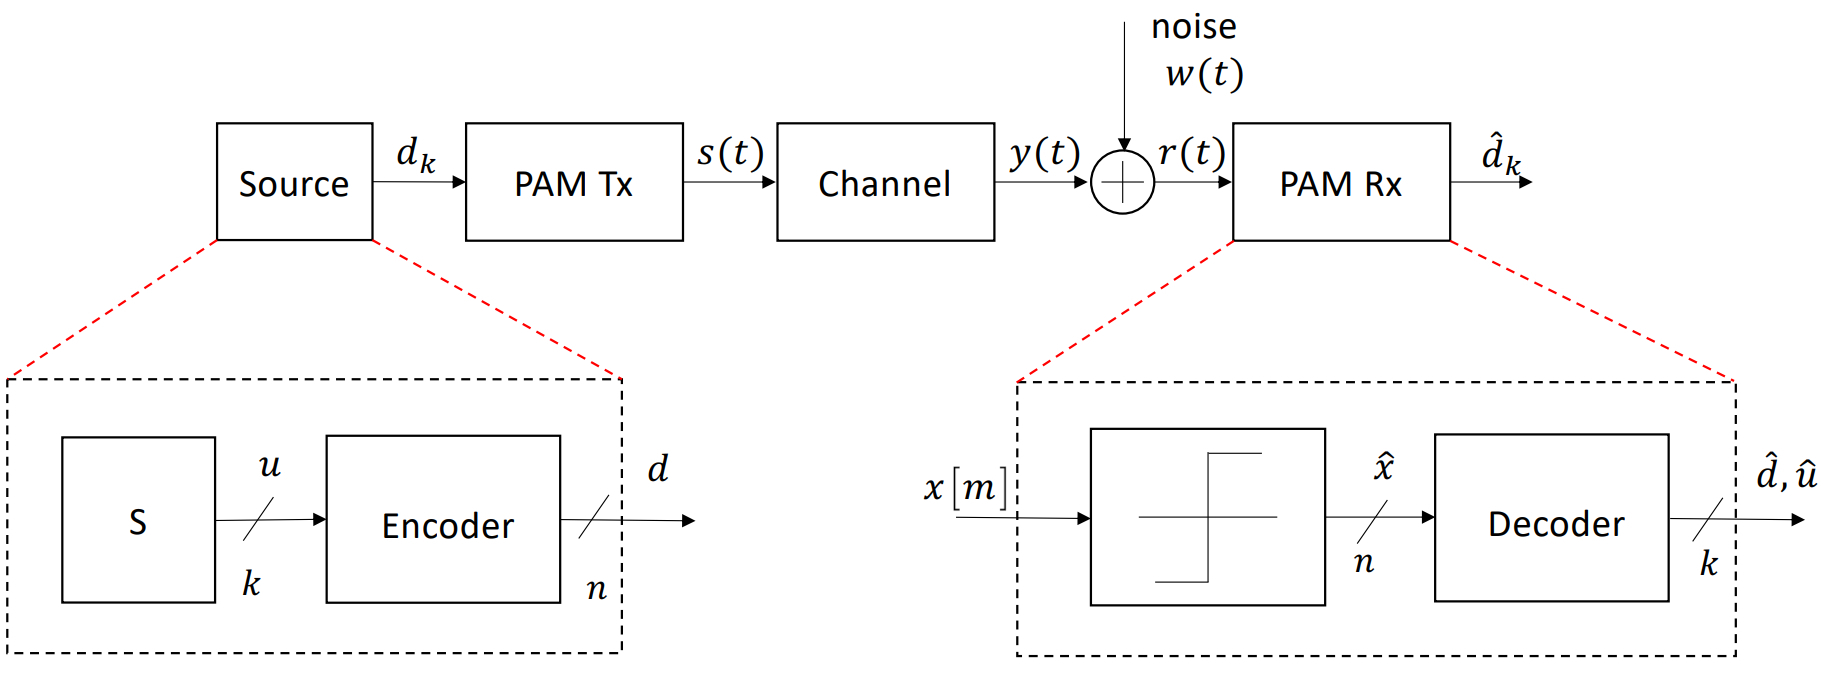
\includegraphics[width=0.675\textwidth]{imgs/encoder_decoder.jpg}
\end{figure}

Sorgente e destinazione introducono \textbf{codificatore} e \textbf{decodificatore} per la gestione dei bit di ridondanza, si può utilizzare lo schema:


\begin{center}
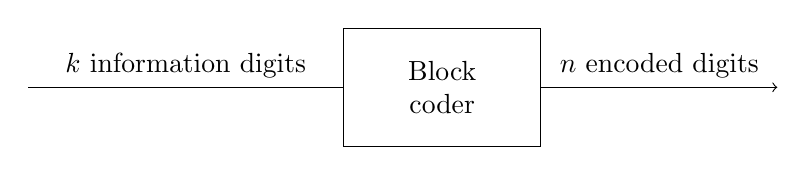
\begin{tikzpicture} [align=center]
    % Draw the block
    
    \node[draw, rectangle, minimum width=2.5cm, minimum height=1.5cm] (block) {Block \\ coder};
    
    % Draw the input arrow
    \draw[-] (block.west) -- ++(-4,0) node[midway, above] {$k$ information digits};
    
    % Draw the output arrow
    \draw[->] (block.east) -- ++(3,0) node[midway, above] {$n$ encoded digits};
\end{tikzpicture}
\end{center}


\begin{center}
    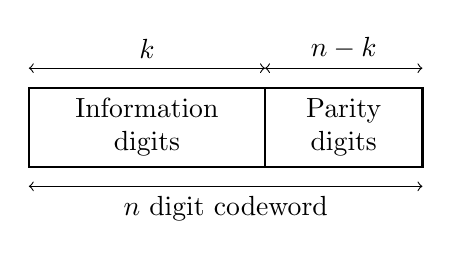
\begin{tikzpicture}[align=center]
    % Draw the main rectangle
    \draw[thick] (0,0) rectangle (5,1);
    
    % Draw the dividing line
    \draw[thick] (3,0) -- (3,1);
    
    % Labels inside the rectangles
    \node at (1.5,0.5) {Information\\digits};
    \node at (4,0.5) {Parity\\digits};
    
    % Arrows and labels
    \draw[<->] (0,1.25) -- (3,1.25) node[midway, above] {$k$};
    \draw[<->] (3,1.25) -- (5,1.25) node[midway, above] {$n-k$};
    \draw[<->] (0,-0.25) -- (5,-0.25) node[midway, below] {$n$ digit codeword};
\end{tikzpicture}

\end{center}
In questo schema l'intero sistema è visto come una componente che aggiunge un errore al messaggio trasmesso.

\paragraph*{Block code}
Si tratta della tipologia più semplice di coding in cui la parola  di codice tramessa è composta da $n-k$ bit di parità.
L'operazione è rappresentabile come operazione di moltiplicazione fra un vettore (parola da trasmettere) e una matrice (\textbf{generator matrix}, definisce il tipo di operazione).

\[
    \mathbf{d} = \mathbf{uG}, \quad \begin{cases}
        \mathbf{d} \text{ coded word} \quad d \in GF(2)^{1 \times n} \\
        \mathbf{u} \text{ parola da trasmettere} \quad u \in GF(2)^{1 \times k} \\
        \mathbf{G} \text{ generator matrix} \quad G \in GF(2)^{k \times n}
    \end{cases}
\]

In generale le prime $k$ colonne della matrice $G$ equiavalgono a $I_k$ (matrice identità $k \times k$) e le restanti $n-k$ colonne sono i bit di ridondanza.
In totale si possono ottenere $2^k$ parole di codice differenti (uscita del codificatore).
Si parla di \textit{coding sistematico} quando i bit di informazione sono semplicemente copiati.

\paragraph*{Error detection}

\begin{center}   
    \begin{tikzpicture}
        % Nodes for the transmitter side
        \node[draw, rectangle, minimum width=1.5cm, minimum height=0.65cm] (T1) at (0,4) {Data 1};
        \node[draw, rectangle, minimum width=1.5cm, minimum height=0.65cm] (T2) at (3,4) {Data 2};
        \node[draw, rectangle, minimum width=1.5cm, minimum height=0.65cm] (T3) at (6,4) {Data 2};
        % create a node containing a red cross
        %\node[draw, cross out, red, thick, minimum size=1cm] (cross) at (4,3) {};
        % create a rotate of 45 degrees
        \node[draw, cross out, red, thick, minimum size=0.5cm, rotate=45] (cross) at (4,3) {};
        % Nodes for the receiver side
        \node[draw, rectangle, minimum width=1.5cm, minimum height=0.65cm] (R1) at (2,2) {Data 1};
        \node[draw, rectangle, minimum width=1.5cm, minimum height=0.65cm] (R2) at (5,2) {Data 2};
        \node[draw, rectangle, minimum width=1.5cm, minimum height=0.65cm] (R3) at (8,2) {Data 2};

        % Arrows for data transmission
        \draw[->, thick] (T1) -- (R1);
        \draw[->, thick] (R1) -- (T2) node[midway, above, sloped] {ACK};
        \draw[->, thick] (T2) -- (R2);
        \draw[->, thick] (R2) -- (T3) node[midway, above, sloped, red] {NACK};
        \draw[->, thick] (T3) -- (R3);

        % Arrow for time
        \draw[<->, dashed] (4.75,1.25) -- (7.75,1.25) node[midway, below] {$T_{ARQ} > T_c$};

        % Vertical lines for transmission boundaries
        \draw[dashed] (4.675,0.5) -- (4.675,3.5);
        \draw[dashed] (7.675,0.5) -- (7.675,3.5);
        
        % Labels for transmissions
        \node at (4.675,0) {1\textsuperscript{st} transmission};
        \node at (7.675,0) {2\textsuperscript{nd} transmission};
        
        % Labels for Transmitter and Receiver
        \node[] at (-2,4) {Transmitter};
        \node[] at (-2,2) {Receiver};
    \end{tikzpicture}
\end{center}



Le tecniche di error detection consistono nel confrontare i bit di ridondanza ricevuti con i bit di ridondanza calcolati utilizzando le parole ricevute. 
Se il confronto ha successo si assume che la trasmissione non abbia introdotto errori, altrimenti si rileva un errore nella trasmissione.
In casi di errore il ricevitore può richiedere una nuova trasmissione, adottando lo schema \textbf{ARQ} (Automatic Repeat reQuest).
In tale schema ad ogni ricezione si risponde con un ACK o un NACK, in base al risultato del confronto.
In caso di NACK si procede con una nuova trasmissione. 
Si tratta di una tecnica di diversità temporale, in quanto la ritrasmissione avviene dopo $T_{ARQ}$, un intervallo temporale superiore al coherence time del canale ($T_{ARQ} > T_c$).
Alcuni ricevitori sono in grado di combinare i due messaggi ricevuti, incrementando la probabilità di ricostruire l'informazione trasmessa.
Una semplice tecnica di error detection è il \textbf{parity check code}, in cui si aggiunge un bit di parità alla fine della parola di 7 bit da trasmettere. Se il numero di bit a 1 è pari, il bit di parità è 0, altrimenti è 1.

\[
    \begin{cases}
        k = 7 \\
        n = 8 
    \end{cases}
    \Rightarrow R = \frac{7}{8},
    \quad \mathbf{G} = \left[I_7, 1_7\right] = 
    \begin{bmatrix}
        1 & 0 & 0 & 0 & 0 & 0 & 0 & 1 \\
        0 & 1 & 0 & 0 & 0 & 0 & 0 & 1 \\
        0 & 0 & 1 & 0 & 0 & 0 & 0 & 1 \\
        0 & 0 & 0 & 1 & 0 & 0 & 0 & 1 \\
        0 & 0 & 0 & 0 & 1 & 0 & 0 & 1 \\
        0 & 0 & 0 & 0 & 0 & 1 & 0 & 1 \\
        0 & 0 & 0 & 0 & 0 & 0 & 1 & 1 \\
    \end{bmatrix}
    \Rightarrow u_7 = \sum_{i=0}^{6} u_i
\]
Il bit di parità è calcolato sommando tutti i bit delle parole usando l'algebra in GF(2).
Sebbene sia molto semplice questa tecnica, non può essere sempre efficace in quanto può riconoscere unicamente un numero di errori dispari, mentre in caso di numero di errori pari si avrà un bilanciamente degli 1 ed il confronto avrà successo.

\paragraph*{Error correction}
Le tecniche di correzione dell'errore sono utilizzate per rilevare e correggere errori di trasmissione, senza necessità di richiedere una nuova trasmissione.
Dato un canale si definisce \textbf{capacità} il massimo rate a cui è possibile trasmettere:
\[
    C = B \log_2(1 + \text{SNR}) \quad \text{bit/s}
\]

Ogni trasmissione con rate $R < C$ ed $\epsilon$ arbitrario è possibile determinare una correzione dell'errore code per cui $P_e < \epsilon$.
Una semplice tecnica di correzione dell'errore è il \textbf{repetition code}, in cui la parola è ripetuta 3 volte. 
Per stabilire quale sia il bit corretto in casi di incongruenza si adotta una strategia maggioritaria.


\[
    \begin{cases}
        k = 1 \\
        n = 3 
    \end{cases}
    \Rightarrow R = \frac{1}{3},
    \quad \mathbf{G} =
    \begin{bmatrix}
        1 & 1 & 1
    \end{bmatrix}
    \quad 
    \begin{cases}
        u = \begin{bmatrix}0\end{bmatrix} \Rightarrow d = \begin{bmatrix}0 & 0 & 0\end{bmatrix} \\
        \\
        u = \begin{bmatrix}1\end{bmatrix} \Rightarrow d = \begin{bmatrix}1 & 1 & 1\end{bmatrix}
    \end{cases}
\]


Questa tecnica è in grado di correggere un unico errore, tuttavia se utilizzato come error detection può rilevare fino a due errori.
La distanza tra due parole di codice è calcolata come numero di bit differenti fra le due stringhe, detta anche \textbf{distanza di Hamming}. Il decodificatore seleziona la parola  con minima distanza rispetto a quella ricevuta.

\[
%\hat{a}_m = \underset{i=1,\ldots,M}{\mathrm{argmin}}
    \hat{d} = \underset{d}{\mathrm{argmin}} \left\{\text{distance}(d, \hat{x})\right\}
\]

Dove $\hat{d}$ è la parola in uscita dal decodificatore, $d$ è una parola possibile e $\hat{x}$ è la parola ricevuta.
Gli errori possono far scegliere al decodificatore la parola sbagliata, la capacità di correzione dell'errore di un codice a blocchi è tanto maggiore quanto maggiore è la distanza di Hamming tra le parola  di codice generabili.
La bontà del codice a blocchi è misurabile con la minima distanza tra parole di codice $d_{min}$.
\[
    d_{min} - 1 \quad \text{Numero massimo di errori rilevabili}
\]

\[
    \left\lfloor \frac{d_{min} - 1}{2} \right\rfloor \quad \text{Numero massimo di errori correggibili}
\]
Maggiore è la distanza di Hamming, maggiore è la ridondanza da aggiungere.
Fissata $R=\frac{k}{n}$, $d_{min}$ sarà più grande al crescere di $k$ e $n$, tuttavia si complica anche il sistema.
\section*{Codici convoluzionali}
I codici convoluzionali, al contrario dei codici a blocchi, non sono sistematici, si trasmettono infatti solo i bit di parità.

Il codificatore utilizza una finestra scorrevole per generare $n>1$ bit di parità, combinando vari sottoinsiemi di bit nel campo GF(2), realizzando una sorta di convoluzione.
Il codificatore si comporta come $n$ filtri lineari in parallelo, i parametri che lo costituiscono sono:
\begin{itemize}
    \item $n$: bit generati
    \item $k$: bit di informazione (si considererà sempre $k=1$)
    \item $L$: lunghezza del vincolo, ovvero il numero di parole di input di $k$ bit che concorrono alla generazione degli $n$ bit di output. Nel caso di $k=1$ sarà la lunghezza dei bit che concorrono alla generazione del codice.
\end{itemize}

La dimensione della finestra corrisponde a $L-k$, quindi si considererà $L-1$. Il codice generato, oltre alla word, è anche funzione dei bit di input precedenti. Ogni bit generato è ottenuto dalla convoluzione in GF(2) con una risposta impulsiva rappresentata da un diverso generatore $g$, di dimensione $kL$.
Possiamo considerare come analogia in $\mathbb{R}$ la convoluzione tra un segnale e la risposta impulsiva di un filtro la cui espressione è:
\[
    y\left[k\right] = \sum_{m=0}^{M-1} g\left[m\right] \cdot x\left[k-m\right]
\]
Per i codici convoluzionali, che operano in GF(2), similmente scriveremo:
\[
    d_j^{\left(i\right)} = \sum_{\ell=0}^{L-1} g_j\left(\ell\right) \cdot u^{\left( i - \ell \right)}
\]

I bit in uscita sono quindi un flusso continuo e non organizzati in blocchi.
Trattandosi di sistemi con memoria, il codificatore può essere rappresentato come una macchina a stati finiti.
L'output del codificatore dipende dal bit in input e dalla stato corrente.
L'evoluzione temporale del codificatore può essere catturata dal diagramma a traliccio (\textit{trellis diagram}), in cui si ha l'evoluzione degli stati in funzione del tempo.
Ogni sequenza, con la corrispondente parola codificata, può essere rappresentata come un cammino nel diagramma a traliccio.
Una trasmissione di $N$ parole di codice implica la trasmissione di $n \cdot N$ bits, ottenuti dalla codifica di $k \cdot N$ input word.
Poiché ogni parola  di codice è funzione anche di $L-1$ parole in input precedenti, la sequenza può essere codificata considerandola solo nella sua interezza. 
Il decodificatore dovrà scegliere la sequenza più "vicina" rispetto a quella ricevuta tra tutte le possibili sequenza, ovvero $2^{k \cdot N}$
\[
    \hat{d} = \underset{d}{\text{argmin}} \left\{\text{distance}(d, \hat{x})\right\}
\]
Dove $d$ è una possibile sequenza, $\hat{x}$ è la sequenza ricevuta e $\hat{d}$ è la sequenza in uscita dal decodificatore.
L'utilizzo nella pratica di codici convoluzionali è stata resa possibile solo dall'introduzione dell'algoritmo di Viterbi, in grado di applicare una decodifica con complessità lineare e non più esponenziale.

\paragraph*{Codice convoluzionale (2, 1, 3)}

In un codice convoluzionale (2, 1, 3), ovvero con parametri $n=2$, $k=1$ e $L=3$, supponiamo di avere come generatori (che si possono dimostrare essere ottimi):
\[
    g_1 = \begin{bmatrix}1 & 1 & 1\end{bmatrix}, \quad g_2 = \begin{bmatrix}1 & 0 & 1\end{bmatrix}
\]

Come si può notare, la dimensione dei generatori è $kL = 1 \cdot 3 = 3$, il code rate è $R = \frac{k}{n} = \frac{1}{2}$, mentre la memoria è $L - 1 = 3 - 1 = 2$.
\begin{center}
    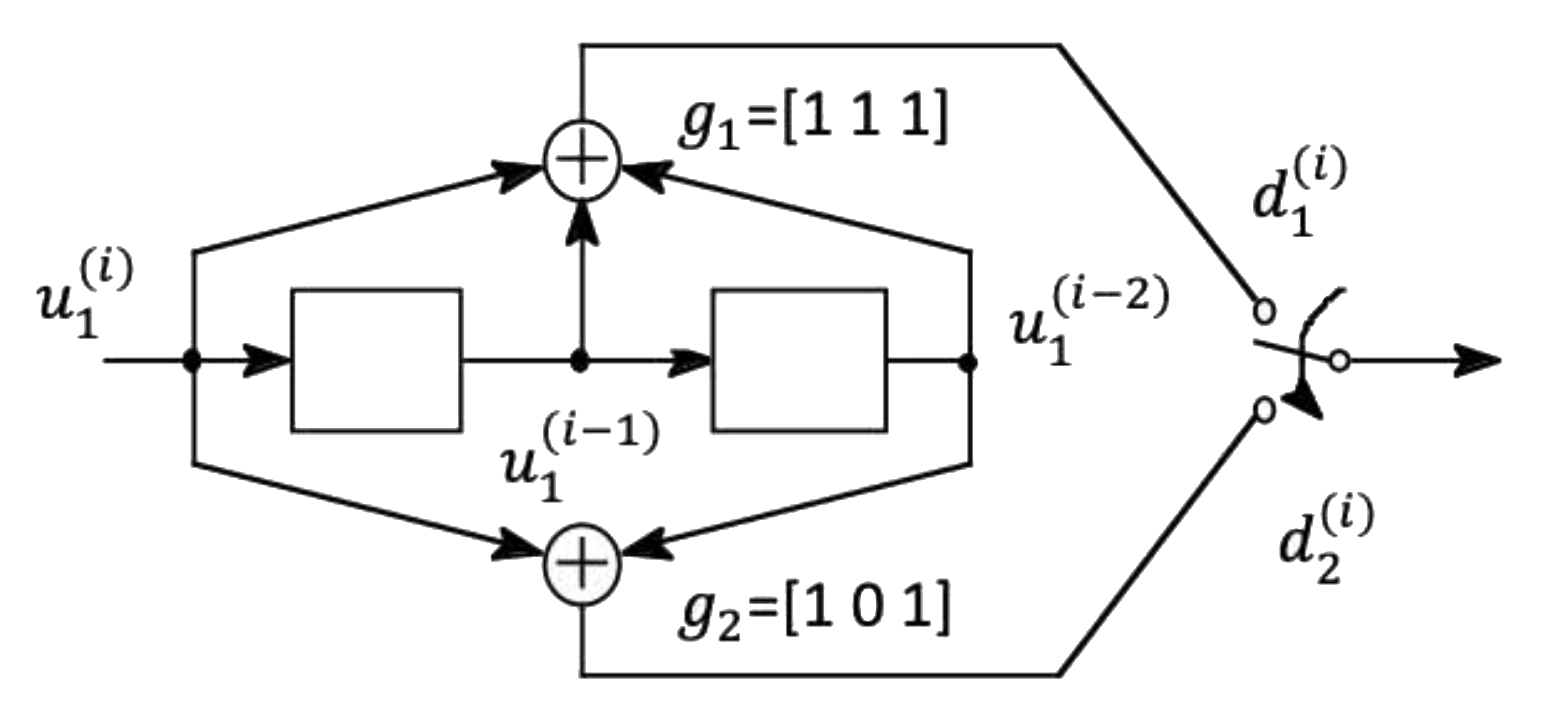
\includegraphics[width=0.5\textwidth]{imgs/213code.png}
\end{center}

Nella figura è possibile notare come siano presenti 2 elementi di memoria (i due rettangoli bianchi), ovvero i $k(L-1)$ elementi di memoria che sono sufficienti a rappresentare lo stato del codificatore.
Le parole di codice di output, applicando quindi la convoluzione tra i bit di input e i generatori, sono:
\[
    d_1^{\left(i\right)} = \sum_{\ell=0}^{2} g_1\left(\ell\right) \cdot u^{\left( i - \ell \right)} = u^{\left(i\right)} + u^{\left(i-1\right)} + u^{\left(i-2\right)}
\]

\[
    d_2^{\left(i\right)} = \sum_{\ell=0}^{2} g_2\left(\ell\right) \cdot u^{\left( i - \ell \right)} = u^{\left(i\right)} + u^{\left(i-2\right)}
\]

Possiamo definire una macchina a stati fatta nella seguente maniera:

\begin{center}
\begin{tikzpicture}[shorten >=1pt, node distance=3cm, on grid, auto]
   \node[state] (q_11)   {11};
   \node[state] (q_10) [below left=of q_11] {10};
   \node[state] (q_01) [below right=of q_11] {01};
   \node[state] (q_00) [below right=of q_10] {00};

    \path[->]
    (q_11) edge [loop above] node {1/10} ()
          edge [bend left=15] node {0/01} (q_01)
    (q_10) edge [bend right=15] node [above] {1/00} (q_01)
          edge [bend left=15] node [right] {1/01} (q_11)
    (q_01) edge [bend left=15] node [right] {0/11} (q_00)
          edge [bend right=15] node [above] {0/10} (q_10)
    (q_00) edge [loop below] node {0/00} ()
          edge [bend left=15] node {1/11} (q_10);
\end{tikzpicture}
\end{center}


Dove i nodi rappresentano lo stato del codificatore, ovvero i bit di memoria, mentre gli archi rappresentano separati dallo slash rispettivamente il bit di input e l'output.
La macchina a stati è ricavabile col seguente codice:

\begin{minted}{python3}
G1 = [True, True, True]
G2 = [True, False, True]

G = [G1, G2]

def next_state(input_bit: bool, state: Tuple[bool, bool]):
    d = [(g[0] & input_bit) ^ (g[1] & state[0]) ^ (g[2] & state[1]) for g in G]
    return (input_bit, state[0]), (d[0], d[1])
\end{minted}

La funzione \texttt{next\_state} prende in input il bit da codificare e lo stato corrente del codificatore, restituendo lo stato successivo, ottenuto con una sorta di shift, e i bit di output.

\paragraph*{Algoritmo di Viterbi}
L'obiettivo è trovare la sequenza con distanza minima rispetto a quella ricevuta:

\[
    \hat{d} = \underset{d}{\text{argmin}} \left( d_H \left(\tilde{d}, \hat{x}\right) \right)
\]
Le possibili sequenza $\tilde{d}$ sono viste come sequenze di $N$ blocchi, ciascuna composta da 
$n$ bit, ovvero i bit prodotti a partire dai $k$ bit di informazione in ingresso alil codificatore.


\[
    d_H\left(\tilde{d}, \hat{x}\right) = \sum_{j=1}^{N} d_H\left(\tilde{d}_j, \hat{x}_j\right)
\]

Dove $d_H$ è la distanza di Hamming tra due sequenze di bit, $\tilde{d}_j$ è la $j$-esima parola  di codice possibile e $\hat{x}_j$ è la $j$-esima parola  di codice ricevuta.
Ogni sequenza $\tilde{d}$ corrisponde ad una seuqenza di stati $\tilde{S}_0, \ldots, \tilde{S}_N$ nel diagramma a trabocco, ovvero a un determinato path. La $j$-esima uscita del codificatore, $\tilde{d}_j$, dipende dalla transizione tra gli stati $\tilde{S}_{j-1}$ e $\tilde{S}_j$.
.
.
.
.

% insert python code hello world hre
La distanza di Hamming può essere calcolata in Python come:
\begin{minted}{python3}
def hamming_distance(a: int, b: int) -> int:
    return bin(a ^ b).count('1')
\end{minted}
Dal diagramma a traliccio possiamo dedurre la funzione di transizione come:
\begin{minted}{python3}

def state_machine(state: int, input_bit: bool) -> Tuple[int, int]:
    match state:
        case 0b01:
            return (0b11, 0b00) if not input_bit else (0b00, 0b10)
        case 0b10:
            return (0b10, 0b01) if not input_bit else (0b01, 0b11)
        case 0b11:
            return (0b01, 0b01) if not input_bit else (0b10, 0b11)
        case 0b00:
            return (0b00, 0b00) if not input_bit else (0b11, 0b10)
        case _:
            raise ValueError("Invalid state")

\end{minted}
Per quanto riguarda invece l'algoritmo di Viterbi, esso può essere definito per sommi capi come:

\begin{minted}{python3}
def viterbi_algorithm(sequence: List[bool]) -> List[bool]:
    # [a_0, a_1, a_2, a_3, ...] -> [a_0 * 2 + a_1, a_2 * 2 + a_3, ...]
    outputs: List[int] = bit_pairs_to_integers(sequence)
    matrix: List[List[Optional[ViterbiCell]]] = populate_matrix(outputs)
    final_state = get_last_state(matrix)
    return get_decoded_sequence(matrix, final_state)
\end{minted}

La funzione \texttt{populate\_matrix} riempie una matrice con celle di Viterbi aggiornando distanze globali e stati successivi per ogni colonna di output. Con il termine output indicheremo l'output del codificatore che abbiamo ricevuto e quindi che dovremo, sfruttano anche lo stato del sistema, trasformare nel bit di input originario, ovvero l'$i$-esimo bit della sequenza che effettivamente si voleva trasmettere. Il numero di riga corrisponde al possibile stato.
\begin{minted}{python3}
def populate_matrix(outputs: List[int]) -> List[List[Optional[ViterbiCell]]]:
    matrix: List[List[Optional[ViterbiCell]]] = empty_matrix(rows=4, cols=len(outputs) + 1)
    matrix[0][0] = ViterbiCell(prev_state=0, global_distance=0, input_bit=False)

    for col in range(len(outputs)):
        target_output = outputs[col]
        for row in range(4):
            current_cell = matrix[row][col]
            if current_cell is None:
                continue
            for input_bit in [False, True]:
                output, next_state = state_machine(row, input_bit)
                new_distance = current_cell.global_distance + hamming_distance(output, target_output)
                next_cell = matrix[next_state][col + 1]
                if next_cell is None or next_cell.global_distance > new_distance:
                    matrix[next_state][col + 1] = ViterbiCell(
                        row, new_distance, input_bit
                    )
    return matrix
\end{minted}

La funzione \texttt{get\_last\_state} trova lo stato finale con la distanza globale minima nell'ultima colonna della matrice.
\begin{minted}{python3}
def get_last_state(matrix: List[List[Optional[ViterbiCell]]]) -> int:
    min_distance = float('inf')
    final_state = None
    last_column = [matrix[i][-1] for i in range(4)]
    for row, cell in enumerate(last_column):
        if cell and cell.global_distance < min_distance:
            min_distance = cell.global_distance
            final_state = row
    return final_state
\end{minted}
La funzione \texttt{get\_decoded\_sequence} ricostruisce la sequenza decodificata risalendo dalla matrice a partire dallo stato finale.
\begin{minted}{python3}
def get_decoded_sequence(matrix: List[List[Optional[ViterbiCell]]], final_state: int) -> List[bool]:
    sequence_length = len(matrix[0]) - 1
    decoded_sequence: List[bool] = [False] * sequence_length
    
    current_state = final_state
    for i in range(sequence_length - 1, -1, -1):
        cell = matrix[current_state][i + 1]
        decoded_sequence[i] = cell.input_bit
        current_state = cell.prev_state

    return decoded_sequence
\end{minted}


Come esempio consideriamo di voler trasmettere la sequenza di bit $010000$, il codificatore emetterà quindi la sequenza $00 \ 11 \ 10 \ 11 \ 00 \ 00$. Supponendo che il decodificatore riceva la sequenza $00 \ 10 \ 10 \ 11 \ 00 \ 00$, l'algoritmo di Viterbi sarà in grado di correggere l'errore e restituire la sequenza corretta $010000$.




\begin{center}
    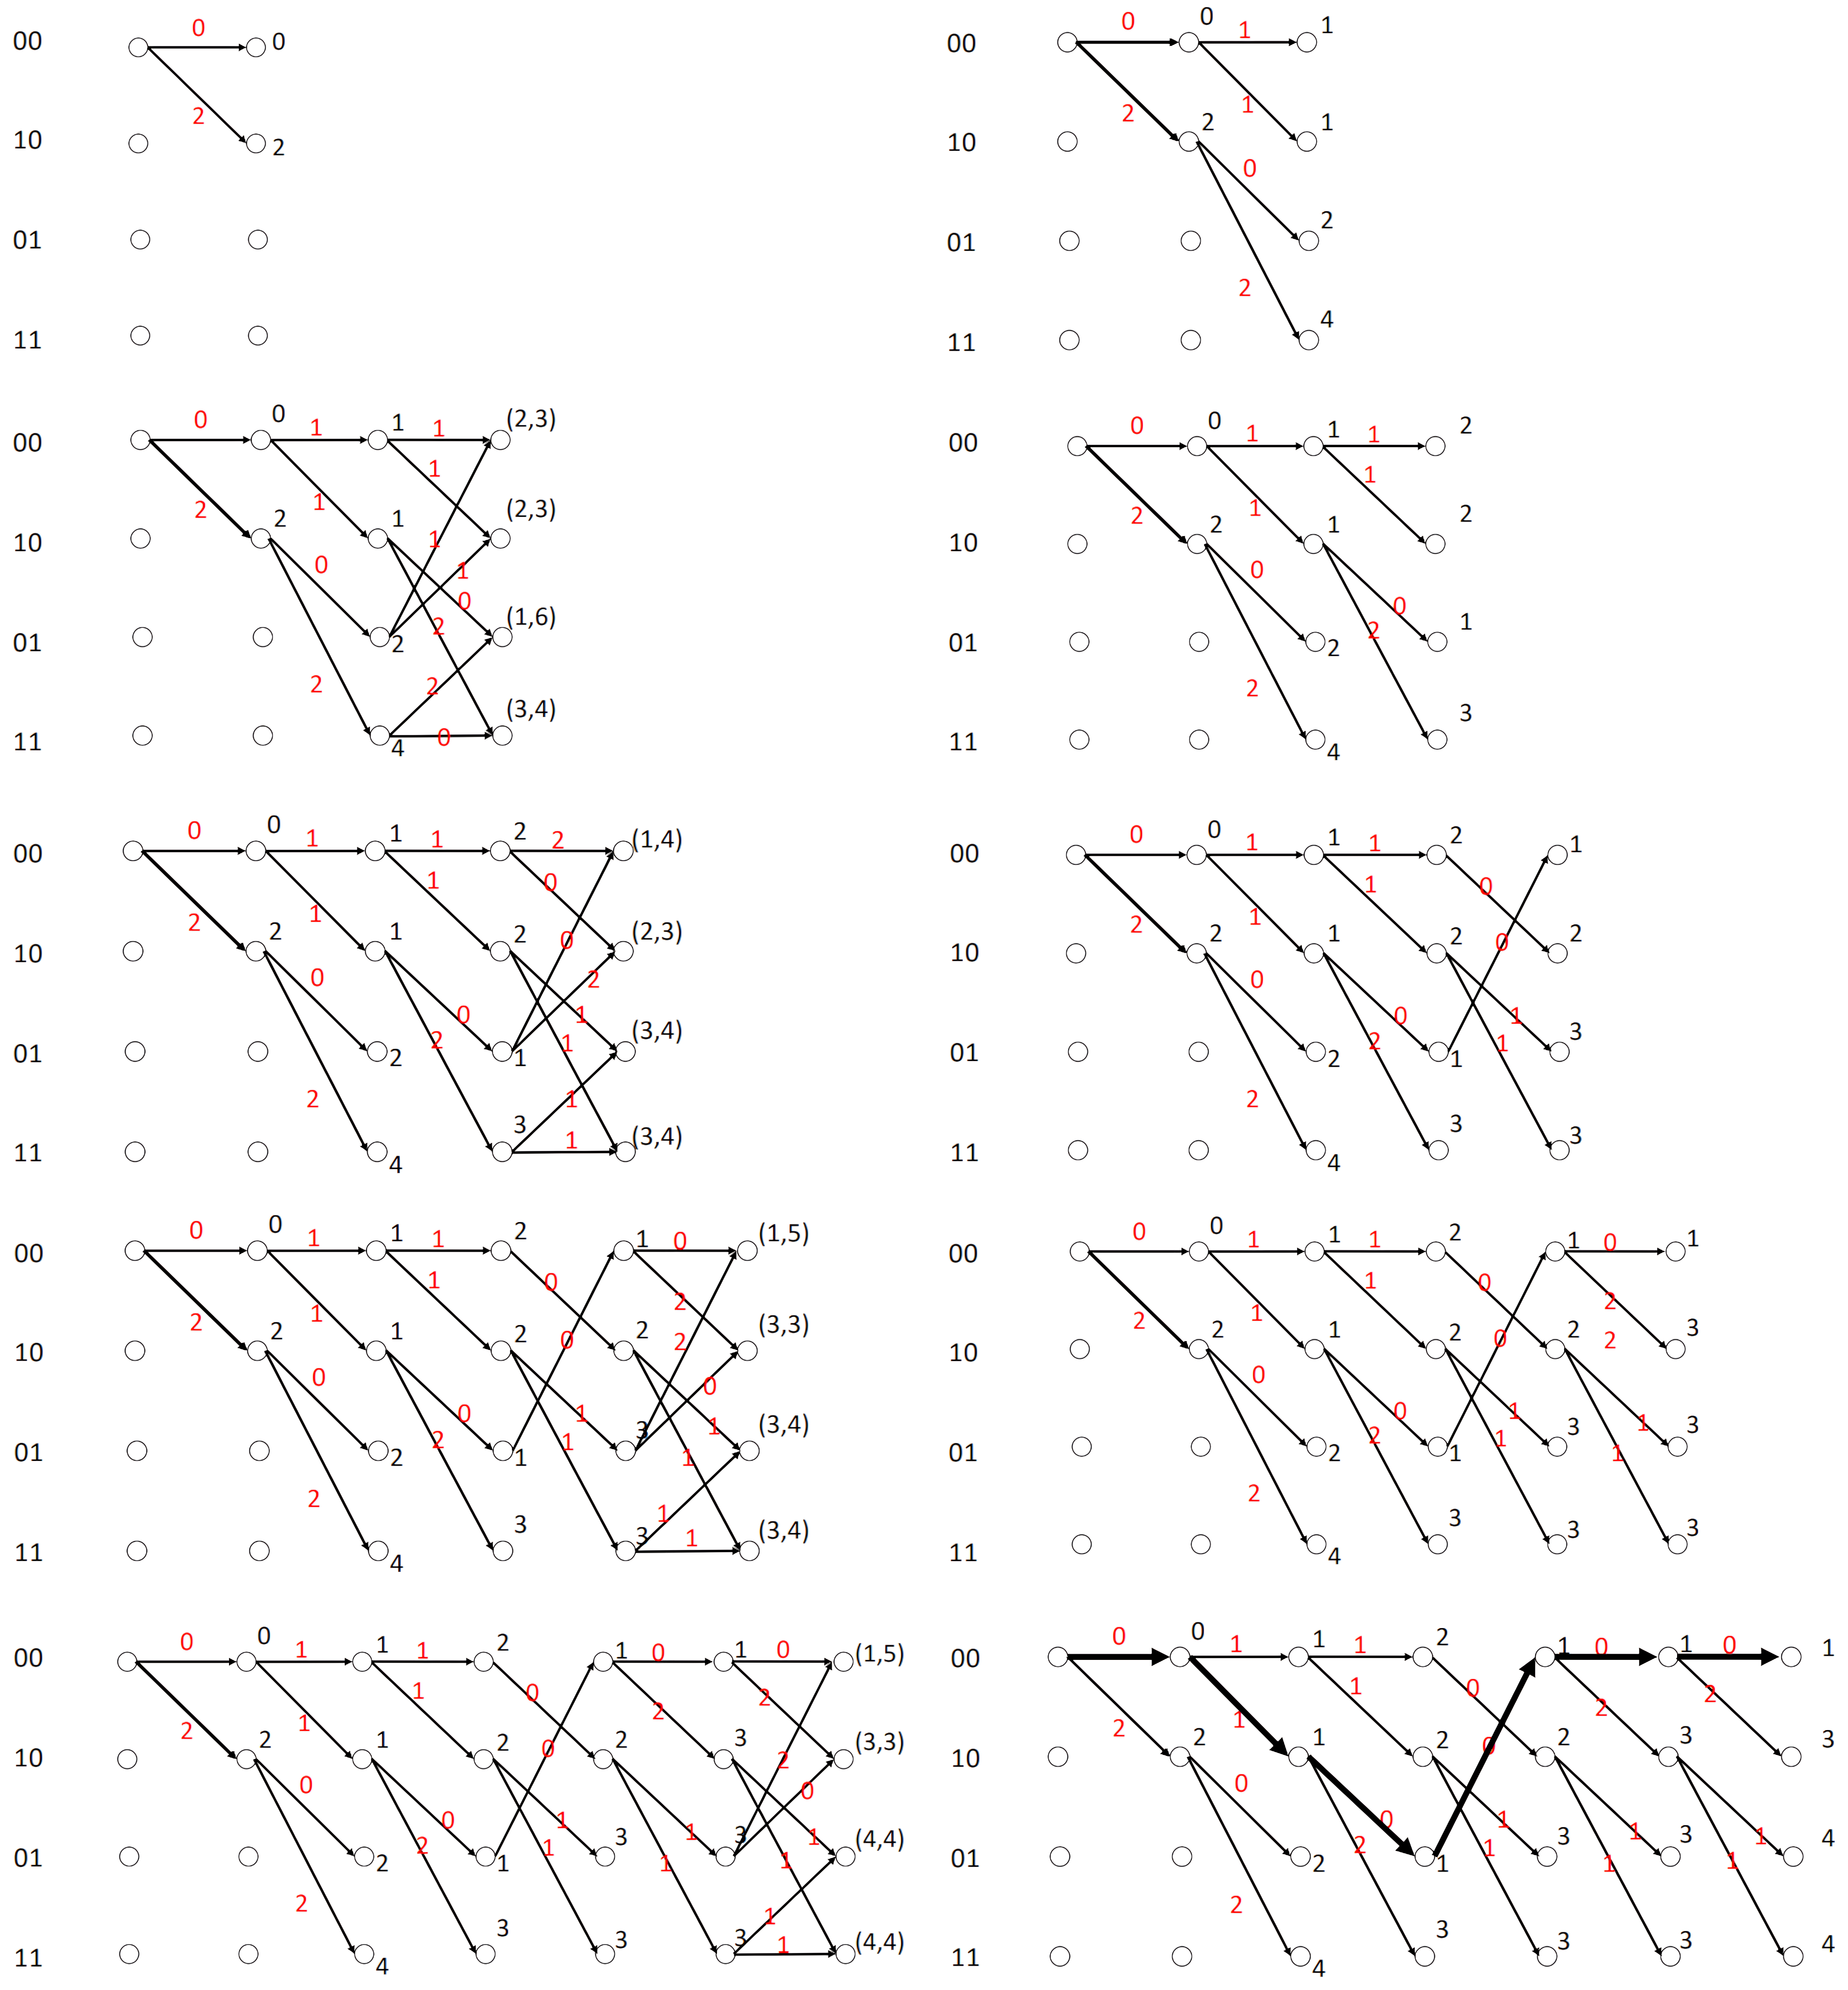
\includegraphics[width=1\textwidth]{imgs/viterbi_example.png}
\end{center}


Ovvero eseguendo l'algoritmo in Python si ottiene la seguente rappresentazione in memoria, stampando i campi \texttt{prev\_state}, \texttt{global\_distance} e \texttt{input\_bit} per ogni cella della matrice:


\begin{table}[h!]

\resizebox{\textwidth}{!}{
    \centering
    \begin{tabular}{|c|c|c|c|c|c|c|c|}
    \hline
    State & Column 1 & Column 2 & Column 3 & Column 4 & Column 5 & Column 6 & Column 7 \\
    \hline
    Row 0b00 & *, 0, * & \textbf{0b00, 0, \textcolor{red}{0}} & 0b00, 1, 0 & 0b00, 2, 0 & \textbf{0b01, 1, \textcolor{red}{0}} & \textbf{0b00, 1, \textcolor{red}{0}} & \textbf{0b00, 1, \textcolor{red}{0}} \\
    \hline
    Row 0b10 & None & 0b00, 2, 1 & \textbf{0b00, 1, \textcolor{red}{1}} & 0b00, 2, 1 & 0b00, 2, 1 & 0b00, 3, 1 & 0b00, 3, 1 \\
    \hline
    Row 0b01 & None & None & 0b10, 2, 0 & \textbf{0b10, 1, \textcolor{red}{0}} & 0b10, 3, 0 & 0b10, 3, 0 & 0b10, 4, 0 \\
    \hline
    Row 0b11 & None & None & 0b10, 4, 1 & 0b10, 3, 1 & 0b10, 3, 1 & 0b10, 3, 1 & 0b10, 4, 1 \\
    \hline
    \end{tabular} 
        
    }
    \end{table}

\section*{Interleaving}



\begin{center}
    \resizebox{\textwidth}{!}{
    \begin{tikzpicture}[node distance=1.5cm, auto, >=Stealth, minimum height=1cm, minimum width=1.5cm]
        % Nodes
        \node[draw, rectangle] (S) {S};
        \node[draw, rectangle, right=of S] (Encoder) {Encoder};
        \node[draw, rectangle, right=of Encoder] (Interleaver) {Interleaver};
        \node[draw, rectangle, right=of Interleaver] (Channel) {Channel};
        \node[draw, rectangle, right=of Channel] (Deinterleaver) {Deinterleaver};
        \node[draw, rectangle, right=of Deinterleaver] (Decoder) {Decoder};
        \node[right=of Decoder, inner sep=0pt, minimum size=0pt] (Uhat) {};

        % Connections
        \draw[->] (S) -- node {$u$} (Encoder);
        \draw[->] (Encoder) -- (Interleaver);
        \draw[->] (Interleaver) -- node {$d$} (Channel);
        \draw[->] (Channel) -- node {$x$} (Deinterleaver);
        \draw[->] (Deinterleaver) -- (Decoder);
        \draw[->] (Decoder) -- node {$\hat{u}$} (Uhat);


        % Dashed boxes
        \draw[dashed] ($(S.north west)+(-0.5,0.5)$) rectangle ($(Interleaver.south east)+(0.5,-0.5)$);
        \draw[dashed] ($(Deinterleaver.north west)+(-0.5,0.5)$) rectangle ($(Decoder.south east)+(0.5,-0.5)$);
    \end{tikzpicture}
}
\end{center}
\begin{center}
    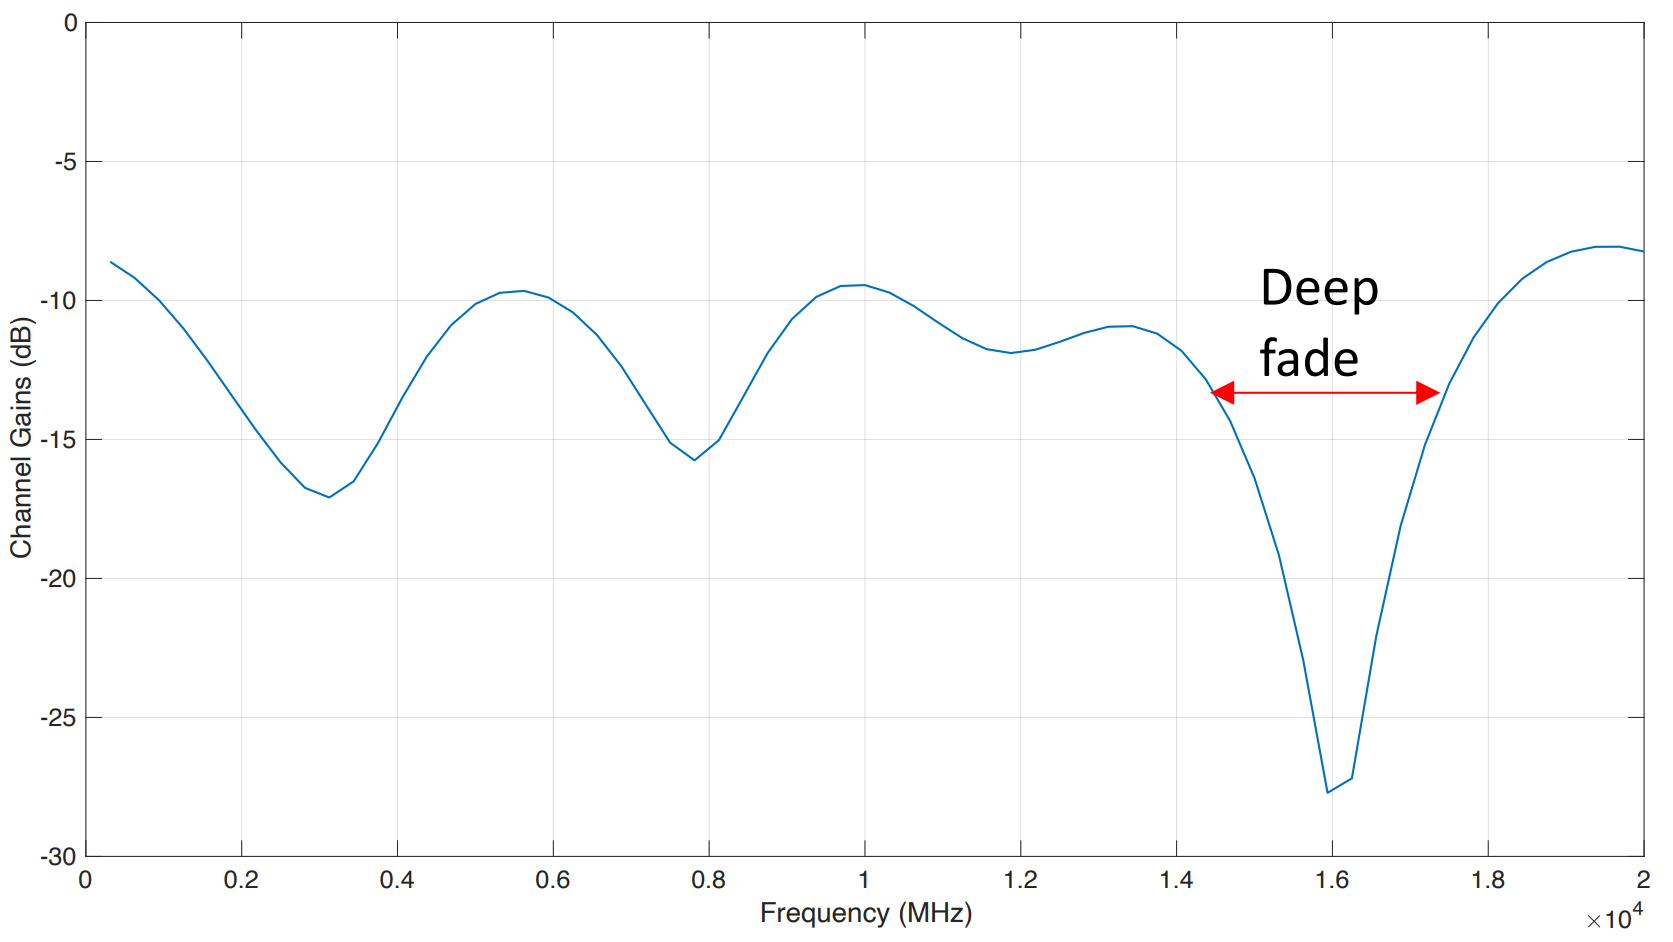
\includegraphics[width=0.5\textwidth]{imgs/deep_fade.png}
\end{center}

I codici convoluzionali risultano adatti per canali memoryless con errori randomici, uniformemente distribuiti ed incorrelati. 
Tuttavia un canale fading è tipicamente soggetto a \textbf{errori a raffica}, ovvero genera un gruppo di errori consecutivi nel tempo e/o in frequenza. 
Quando il canale è in \textbf{deep fade} ci sono delle dipendenze statistiche tra errori consecutivi.
L'idea dell'interleaving consiste nel far sembrare il canale senza memoria dal punto di vista del decodificatore, de-correlando gli errori provocati dal canale, semplicemente rimescolando i bit prodotti del codificatore prima di effettuare la trasmissione.
Lato ricevitore prima del decodificatore verrà effettuata un'operazione di de-interleaving per ripristinare l'ordine originale.
Il costo delle operazioni di (de-)interleaving è pagato in termini di latenza in quanto sia lato ricevitore che lato trasmettitore è necessario avere un intero blocco di dati prima di poter effettuare le operazioni. 
Esiste un trade-off tra latenza e decorrelazione ottenibile, basata sulla profondità $k$ dell'interleaver, ovvero la dimensione del blocco sul quale si effettua l'operazione di rimescolamento.

Per esempio disponendo una sequenza dentro una matrice, possiamo ottenere un interleaver considerando la trasposta:
\begin{table}[h!]
    \centering
    \begin{tabular}{c}
    
    \begin{tabular}{|c|c|c|c|}
    \hline
    A & B & C & D \\ \hline
    E & F & G & H \\ \hline
    I & J & K & L \\ \hline
    M & N & O & P \\ \hline
    \end{tabular}
    
    \quad $\rightarrow$ \quad
    
    \begin{tabular}{|c|c|c|c|}
    \hline
    A & E & I & M \\ \hline
    B & F & J & N \\ \hline
    C & G & K & O \\ \hline
    D & H & L & P \\ \hline
    \end{tabular}
    
    \end{tabular}
\end{table}
   

\begin{center}
    \resizebox{\textwidth}{!}{
    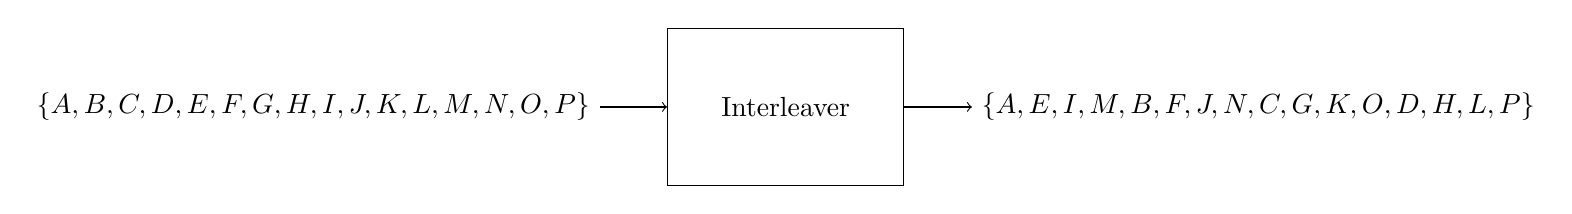
\begin{tikzpicture}
        \node (input) at (0,0) {$\{A,B,C,D,E,F,G,H,I,J,K,L,M,N,O,P\}$};
        \node[draw, minimum height=2cm, minimum width=3cm, align=center] (interleaver) at (6,0) {Interleaver};
        \node (output) at (12,0) {$\{A,E,I,M,B,F,J,N,C,G,K,O,D,H,L,P\}$};

        \draw[->] (input) -- (interleaver);
        \draw[->] (interleaver) -- (output);
    \end{tikzpicture}
    }
\end{center}



\paragraph*{Turbo code e LDPC (Low Density Parity Check)}
Nella formula della capacità del canale di Shannon\footnote{$C=B\log_2(1+\text{SNR}) \si{b/s}$} il rate $R = \frac{k}{n}$ prevede sia $k$ che $n$ tendenti all'infinito, tuttavia la lunghezza del codice nei sistemi reali è finito, quindi ciò che si ottiene è una performance lontana da quella teorica. 
Negli anni sono stati introdotti nuovi codici, sempre più efficienti, tra cui turbo code e LDPC, i quali si avvicinano al limite teorico imposto dalla formula di Shannon.


%Più nel dettaglio abbiamo lato trasmettitore da eseguire i seguenti passi:

\begin{center}
    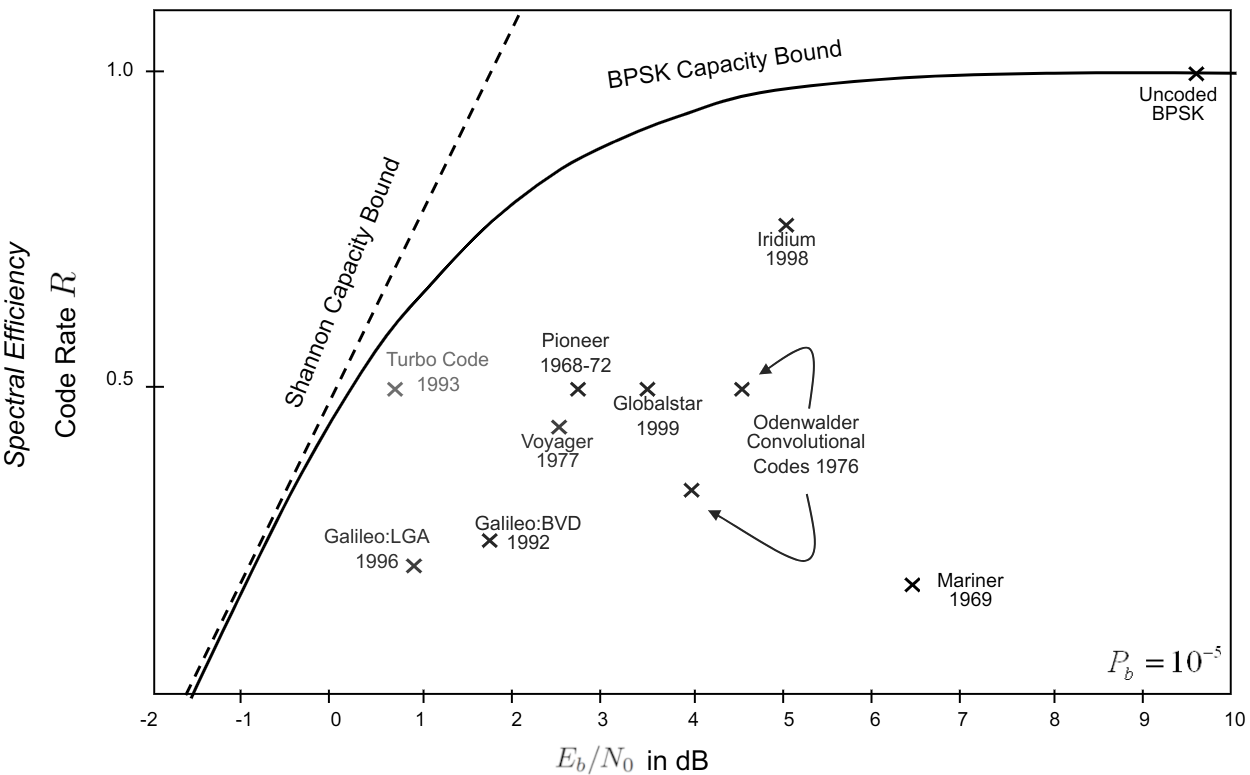
\includegraphics[width=0.75\textwidth]{imgs/codes_and_shannon_bound.png}
\end{center}
\paragraph*{Turbo code (correzione dell'errore)}

Si tratta di un codice convoluzionale in cui sono utilizzati due codificatori in parallelo in grado di generare due sequenze indipendenti, migliorando il processo di decodifica grazie alla ridondanza ottenuta e alla diversità, ottenuta dalla presenza di uno stream di dati differente.
Il sistema è composto da tre sequenze di cui due codificate e una inalterata. L'utilizzo dell'interleaver permette di estendere artificialmente la lunghezza della sequenza, avvicinandosi alle ipotesi di Shannon. Inoltre l'interleaver permette di ottenere sequenze indipendenti. 
Il trasmettitore invia quindi tre sequenze, tra cui quella originaria, ottenendo un $R=\frac{1}{3}$. L'idea è che se il canale produce un errore le due sequenze prodotte in maniera differente possono essere unite  per correggere l'errore.
Per quanto riguarda il decodificatore si utilizzano due decodificatori in cascata, il primo prevede in ingresso i bit sistematici e la prima sequenza generata senza interleaving. L'output prodotto invece di essere utilizzato come uscita del sistema è inviato ad un inteleaver, assieme ai bit sistematici. 
Le due sequenze dopo l'interleaving sono mandate in ingresso, assieme alla seconda sequenza di parità, al secondo decodificatore. L'uscita è infine inviata al deinterleaver. 
Completato il primo ciclo è possibile effettuarne altri, mandando nuovamente in ingresso al primo decodificatore l'uscita dell'interleaver. 
L'uscita dei decodificatori rappresenta una stima, sempre più accurata, della sequenza trasmessa. Il processo iterativo va avanti finché vi sono modifiche nei bit decifrati.
In generale se il SNR rispetta le condizioni di Shannon l'impiego di turbo codes permette di effettuare la correzione degli errori ed ottenere dei BER molto bassi, tuttavia il prezzo è ancora pagato in termini di latenza.






\begin{center}
        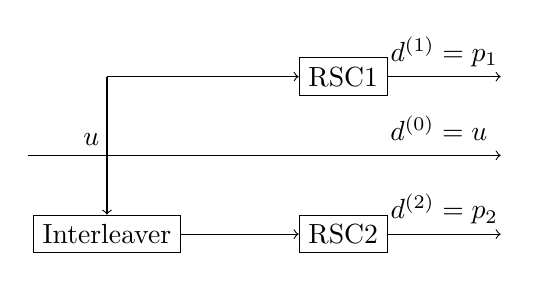
\begin{tikzpicture}
            % Draw blocks
            \node[draw, rectangle] (RSC1) at (3,2) {RSC1};
            % dummy node for alignment
            \node[inner sep=0pt, minimum size=0pt] (dummy) at (3,1) {};
            \node[draw, rectangle] (Interleaver) at (0,0) {Interleaver};
            \node[draw, rectangle] (RSC2) at (3,0) {RSC2};
            
            \draw[->] (0,2) -- (RSC1) node[midway, above] {};
            \draw[->] (RSC1) -- (5,2) node[midway, above] {$d^{(1)} = p_1$};
            \draw[->] (Interleaver) -- (RSC2);
            \draw[->] (RSC2) -- (5,0) node[midway, above]{$d^{(2)} = p_2$}; 
            \draw[->] (-1,1) -- (5,1) node[midway, above, xshift=63, yshift=2] {$d^{(0)} = u$};
            \draw[<-] (Interleaver) -- (0, 2) node[midway, left] {}; 
            \node at (-0.2,1.2) {$u$};
        \end{tikzpicture}
\end{center}
\begin{enumerate}
    \item I bit di informazione (e.g. $01101$) entrano nel trasmettitore e vengono copiati negli codificatore RSC1 e RSC2, che corrispondono a codici diversi. Prima di entrare in RSC2, i bit di informazione vengono rimescolati dall'interleaver (e.g. $10011$).
    \item Ogni codificatore genera una stringa di bit di correzione di errore (bit di parità) eseguendo una serie di calcoli sui bit di informazione che riceve (e.g. rispettivamente, $10110$ e $11100$).
    \item I bit di informazione e le due stringhe di bit di parità sono combinati in un unico blocco e inviati sul canale, dove il rumore può causare errori nella trasmissione.
\end{enumerate}

Per quanto rigurda la ricezione, il processo è il seguente:

\begin{center}
    \begin{tikzpicture}[node distance=1.5cm, auto, >=Stealth, minimum height=1cm, minimum width=1.5cm]

        \node[draw, rectangle] (D1) at (3,0) {D1};
        \node[draw, rectangle] (I) at (6,0) {Interleaver};
        \node[draw, rectangle] (D2) at (9,0) {D2};
        \node[draw, rectangle] (InvI) at (6,2) {Inv(Interleaver)};

        \draw[->] (0,0) -- (2.25, 0) node[midway, above] {$\hat{p}_1$};
        \draw[->] (0,-0.875) -| (D1) node[midway, below] {$\hat{u}$};
        \draw[->] (0,-1.75) -| (D2) node[midway, below] {$\hat{p}_2$};
        \draw[->] (3,-0.875) -| (5.675, -0.5) node[midway, below] {};
        \draw[->] (D1) -- (I) node[midway, above] {Le12};
        \draw[->] (I) -- (D2);
        \draw[->] (D2) |- (InvI) node[midway, right] {Le21};
        \draw[->] (InvI) -| (D1);
    \end{tikzpicture}
\end{center}



\begin{enumerate}
    \item Al segnale (campionato) viene associata una lista di interi (e.g. $[7, -5, 5, 2, -4; \ 6, 5, 7 -2, \textcolor{red}{-2}; \ 3, 8, 1, -5, -3]$, dove $\hat{p}_1$, $\hat{u}$ e $\hat{p}_2$ sono stati separati da un punto e virgola, mentre il rosso è indicata una predizione sbagliata), 
    i cui elementi indicano quanto è probabile che un bit sia 0 o 1. 
    Ad esempio, -7 significa che il bit è quasi certamente uno 0, mentre +7 significa che è quasi certamente un 1. 
    Notare che un errore è avvenuto nel quinto bit del blocco: originariamente un 1, ora ha un valore negativo, che suggerisce uno 0 logico.
    \item Ogni decodificatore prende la lista contenente l'informazione con rumore e la rispettiva lista di parità e calcola quanto è sicuro di ciascun bit decodificato (\textit{reliability values}).
    La lista di affidabilità in uscita dal primo decodificatore è sfruttata dall'interleaver. I due decodificatori si scambiano queste informazioni di affidabilità ripetutamente e dopo un certo numero di iterazioni, tipicamente da quattro a dieci, iniziano ad essere d'accordo su tutti i bit decodificati. 
    Nella prima iterazione il primo decodificatore usa i bit sistematici, dalla seconda userà i bit di affidabilità.
    \item I dati decodificati sono la somma della lista contenente l'informazione (con rumore, e.g. $[6, 5, 7 -2, \textcolor{red}{-2}]$) più le due liste finali contenti i valori di confidenza(e.g. $[-5, 3, 7, -6, 5]$ e $[-3, 4, 2, -4, 3]$).
    L'output ($[-14, 12, 16, -12, 6]$) viene convertito nuovamente in bit binari ($[0, 1, 1, 0, 1]$,  da cui si può notare che il quinto bit ora ha il valore corretto).
\end{enumerate}



\begin{center}
    
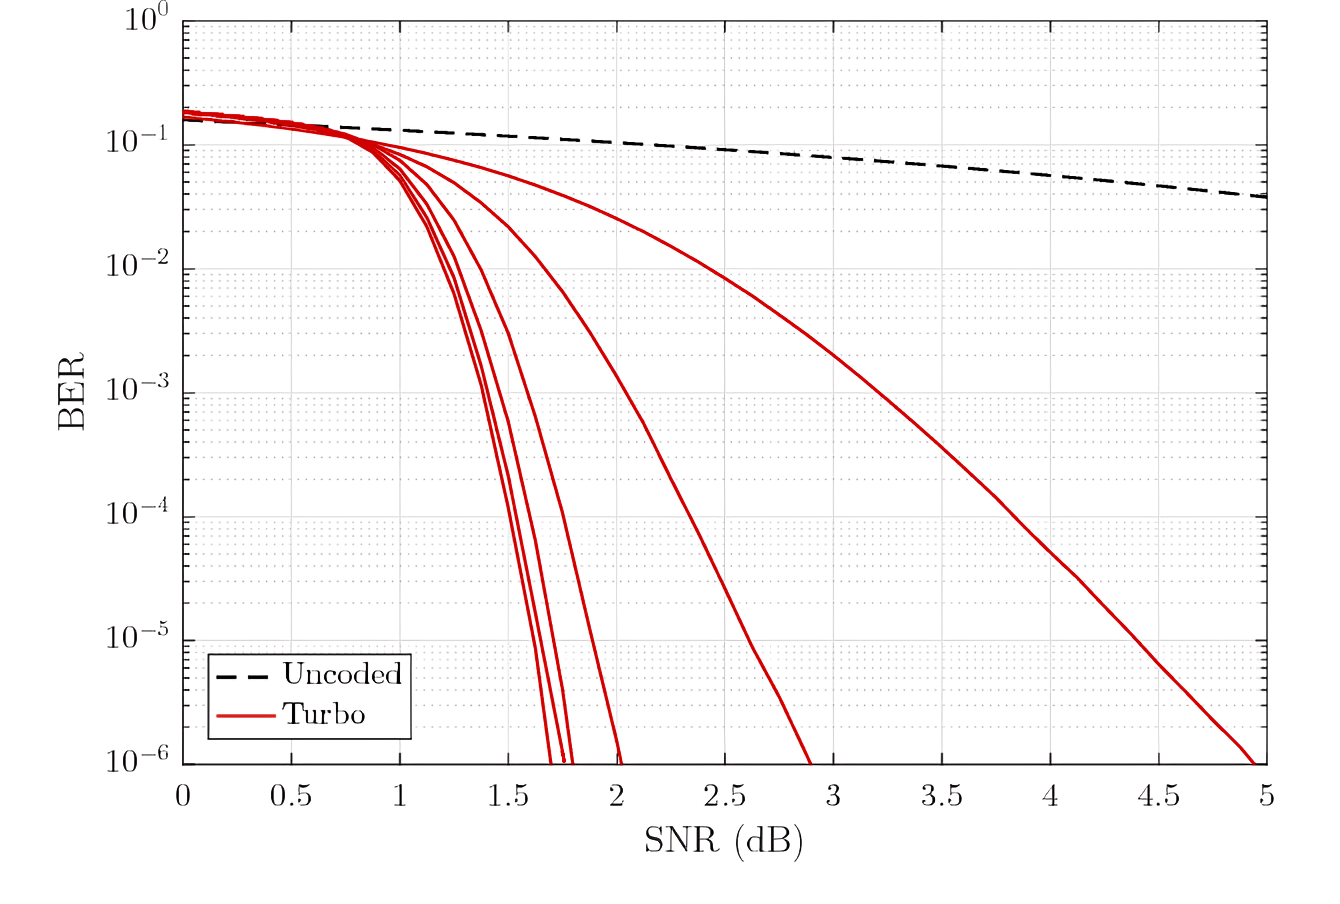
\includegraphics[width=0.5\textwidth]{imgs/turbo_code_ber.png}
\end{center}

In figura viene mostrata la convergenza con $K=2048$, $R=1/2$ e un numero di iterazioni, da sinistra a destra, pari rispettivamente a $32, 16, 8, 4, 2, 1$.


\section*{Diversità spaziale}

In generale sia la diversità in tempo che il frequenza richiedono parecchie risorse, per questo un altro tipo di diversità è spesso sfruttata, semplicemente utilizzando più antenne. Si possono sfruttare due tipologie di guadagni differenti:
\begin{itemize}
    \item \textbf{Guadagno di array}: si tratta del guadagno di potenza ottenuto utilizzando più antenne rispetto all'utilizzo della singola antenna. Il guadagno è tanto più alto quanto è alta la correlazione spaziale del canale. Si sfruttano tipicamente antenne direzionali.
    \item \textbf{Guadagno di diversità}: si tratta del guadagno ottenuto combinando i segnali ricevuti dalle varie antenne, considerati incorrelati. Tale guadagno è massimo quando i segnali sono completamente decorrelati, e deriva dal fatto che l'SNR all'uscita del combinatore ha una distribuzione statistica più "favorevole" rispetto al caso di un singolo cammino.
\end{itemize} 

Per assumere incorrelazione tra le varie antenne la loro distanza deve essere almeno la metà della lunghezza d'onda:
\[
    d_c = \frac{\lambda}{2} \quad \text{distanza di coerenza}
\]  

La \textbf{distanza di coerenza} deriva dalle proprietà di tempo varianza del canale, tuttavia come si può osservare non ha dipendenze né dal tempo, né dalla velocità.

Le frequenze portanti attualmente utilizzate permettono di utilizzare anche antenne nel solito sistema sfruttando al massimo la diversità spaziale.
Bisogna comunque tenere in considerazione che ogni antenna ha bisogno della propria catena RF, quindi lo spazio occupato è maggiore rispetto alla grandezza dell'antenna.


\paragraph*{Canale MIMO (Multiple Input Multiple Output)}


Nei classici sistemi con un antenna in trasmissione ed un'antenna in ricezione, il canale, se a banda stretta può essere descritto da uno scalare complesso.
Nel caso di sistemi con più antenne in trasmissione e ricezione tra ogni coppia di antenne vi è un canale differente, quindi l'intero sistema, per quanto riguarda il canale, può essere descritto tramite una matrice complessa.
\[ 
    \mathbf{H} = 
    \begin{bmatrix}
        h_{11} & h_{12} & \ldots & h_{1M} \\
        h_{21} & h_{22} & \ldots & h_{2M} \\
        \vdots & \vdots & \ddots & \vdots \\
        h_{N1} & h_{N2} & \ldots & h_{NM} \\
    \end{bmatrix}
    , \quad
    \begin{array}{ll}
            \mathbf{H} \in \mathbb{C}^{N \times M} \\
            \mathbf{y} = \mathbf{Hx} 
    \end{array}
\]

Dove $\mathbf{x}$ è il segnale trasmesso, $\mathbf{y}$ è il segnale ricevuto e $\mathbf{H}$ è la matrice del canale. In questo caso, $N$ rappresenta il numero di antenne in ricezione mentre $M$ il numero di antenne in trasmissione.
\paragraph*{Canale SIMO (Single Input Multiple Output)}
\begin{center}
    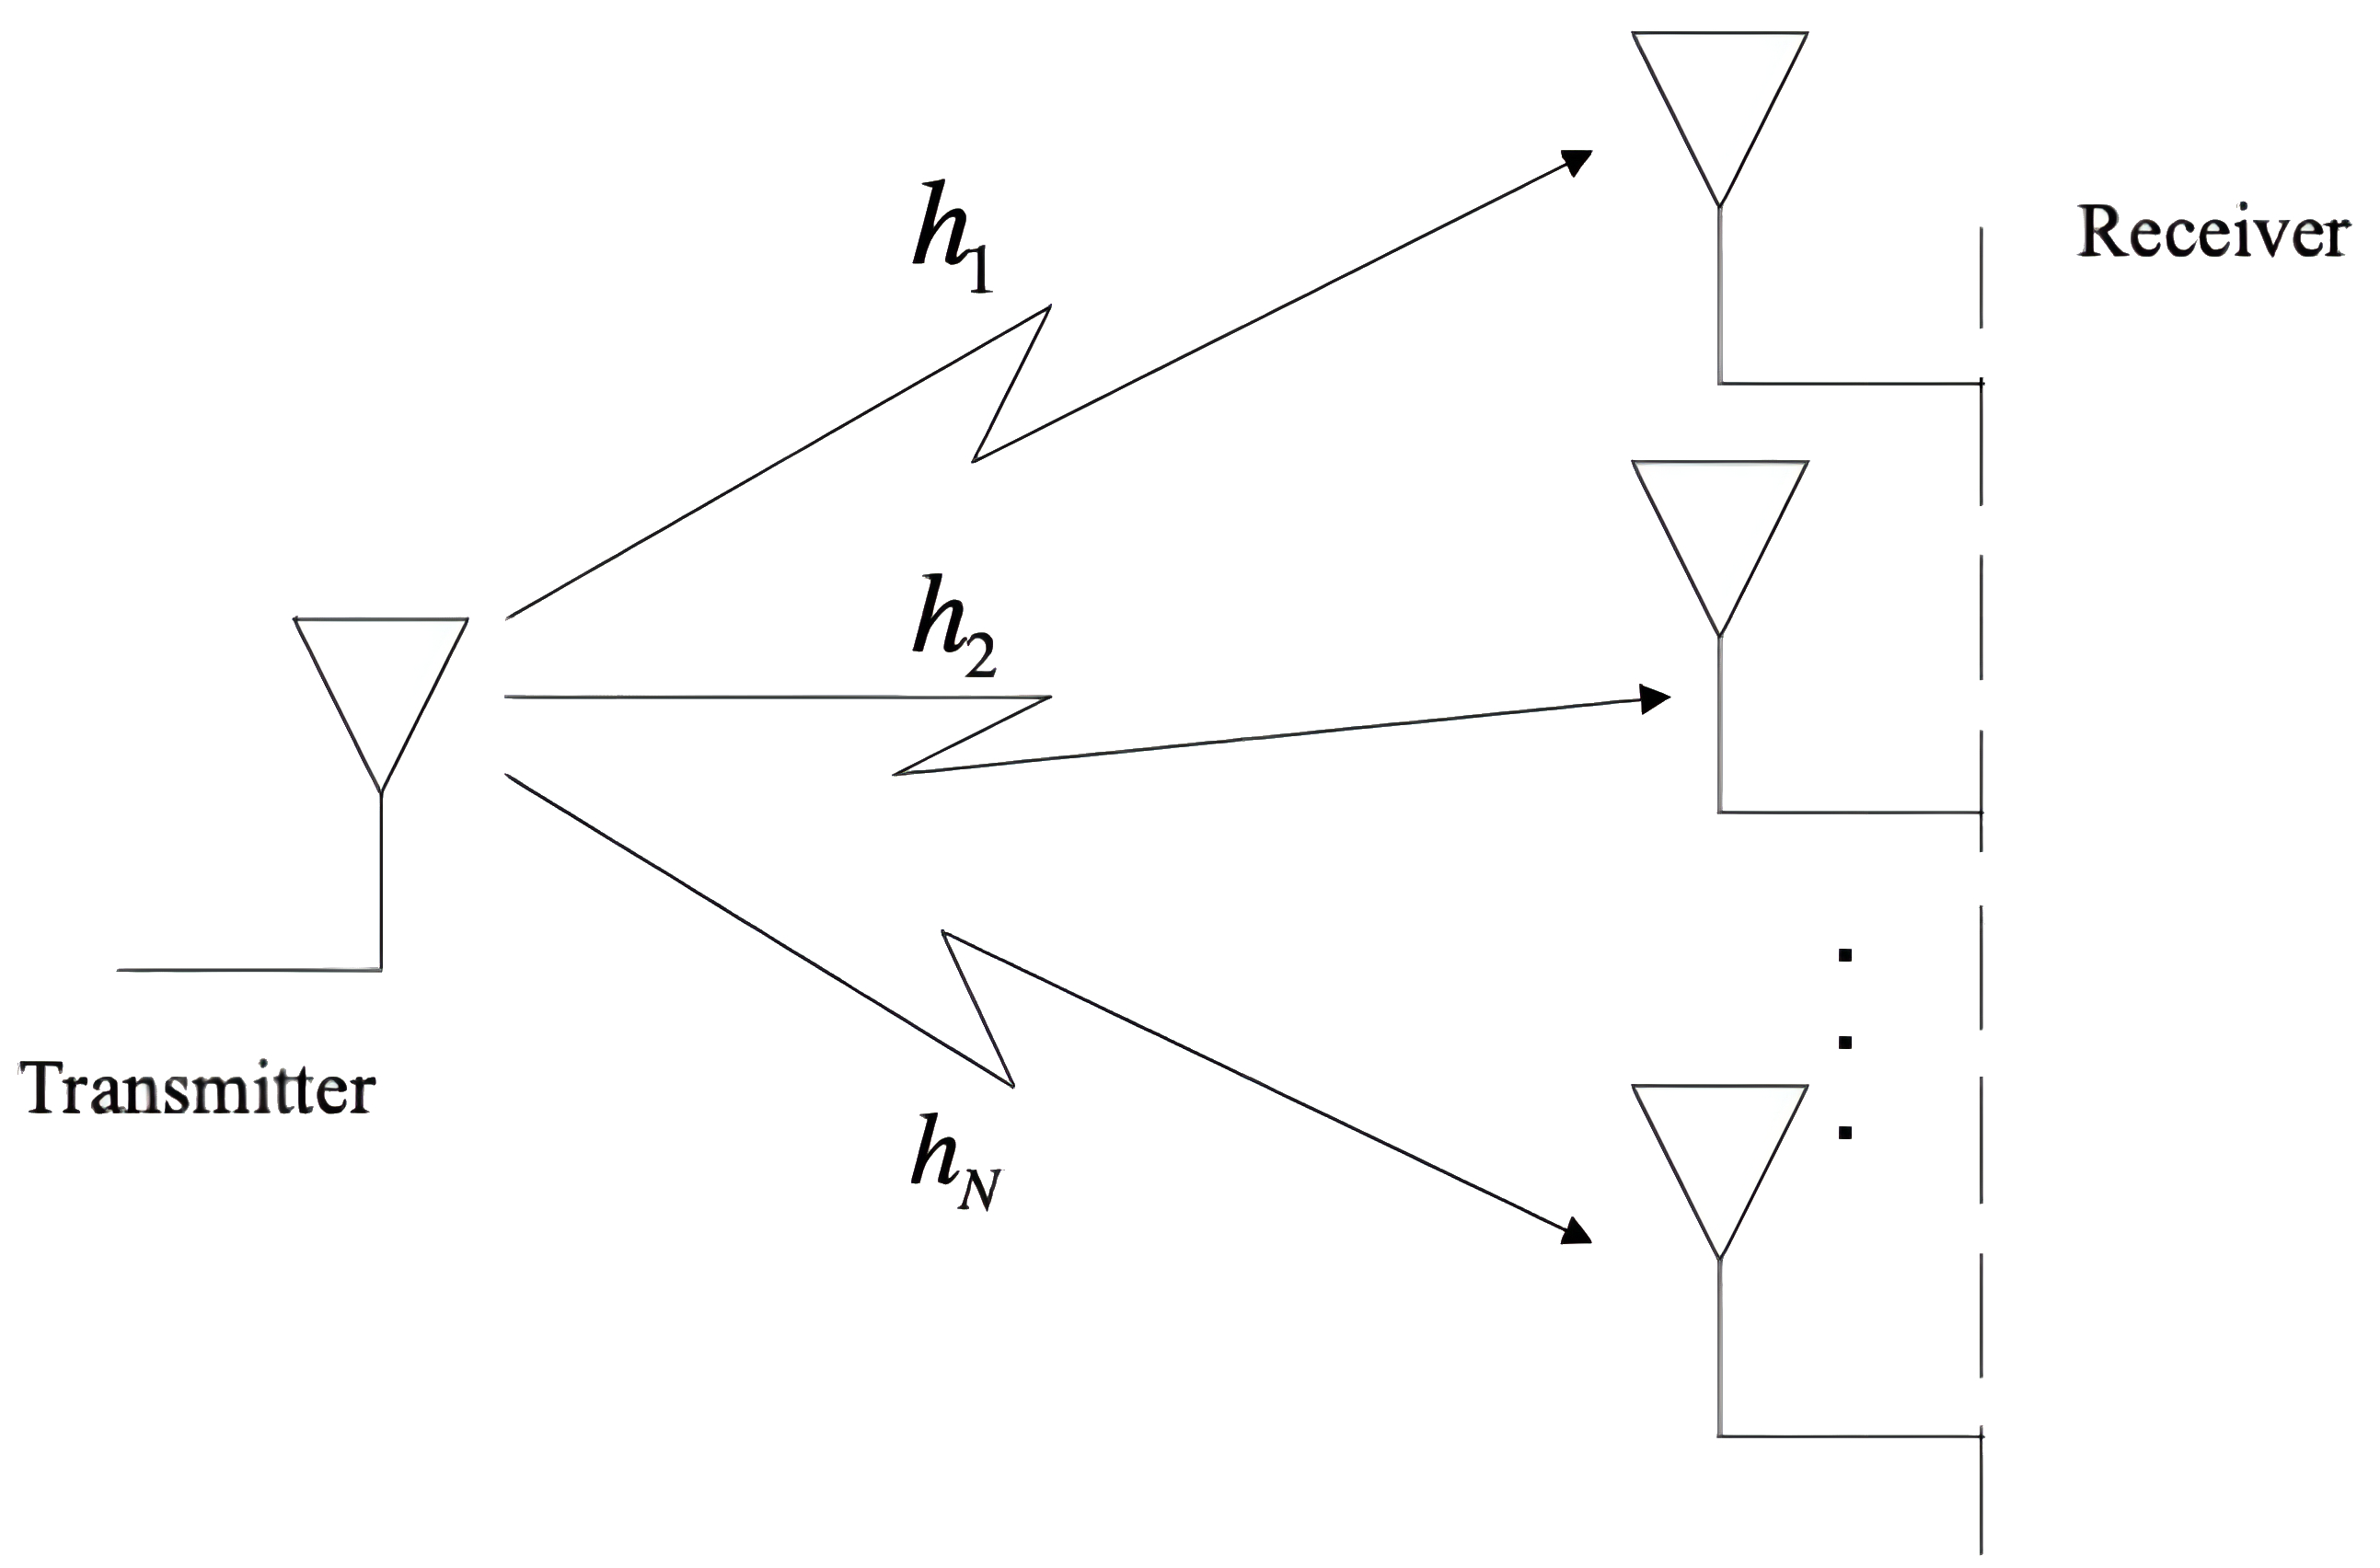
\includegraphics[width=0.4\textwidth]{imgs/simo.jpg}
\end{center}
Nel caso di un'unica antenna in trasmissione si parla di canale SIMO ed in tal caso $\mathbf{H} \in \mathbb{C}^{N \times 1}$
\[
    y_i[m] = h_i c_m + n_i[m] \quad i = 1, \ldots, N
\]
Questo rappresenta il segnale ricevuto sull'$i$-esima antenna.
Ogni segnale ha il proprio rumore e distorsione da parte del canale.
Possiamo per i calcoli assumere che $h_i$ sia una costante, perché nonostante sia modellizzata come una variabile aleatoria, ne faremo una stima misurando il canale, per un tempo che dovrà essere maggiore del symbol time.

L'idea più semplice per sfruttare la diversità è scegliere di volta in volta il segnale con attenuzione minore, stimando il canale.
Tuttavia esistono tecniche in grado di utilizzare le informazioni provenienti da tutti i segnali ricevuti.
% TODO: i %w_i sono reali o complessi 
%\[
%    z[m] = \sum_{i=1}^{N} w_i x_i[m] = \sum_{i=1}^{N} w_i h_i c_m + \sum_{i=1}^{N} w_i n_i[m]
%\]

\[
    z[m] = \mathbf{w}^H \mathbf{y}[m] = \mathbf{w}^H \mathbf{h} x[m] + \mathbf{w}^H \mathbf{n}[m] = \mathbf{w}^H \mathbf{h} c_m + \mathbf{w}^H \mathbf{n}[m]
\]
dove $w_i$ sono i pesi assegnati alle varie antenne.


%\[
%    P = \mathbb{E} \left[ \left| \sum_{i=1}^{N} w_i h_i c_m  \right|^2 \right] = \mathbb{E} \left[  |c_m|^2  \right] \left| \sum_{i=1}^{N} w_i h_i \right|^2 = A \left| \sum_{i=1}^{N} w_i h_i \right|^2 = A \left| \mathbf{w}^T \mathbf{h} \right|^2
%\]
\[
    %P = \langle \mathbf{w}^H \mathbf{h} c_m, \mathbf{w}^H \mathbf{h} c_m \rangle
    P = \mathbb{E} \left[ | \mathbf{w}^H \mathbf{h} c_m |^2 \right]= \mathbb{E} \left[ |c_m|^2 \right] | \mathbf{w}^H \mathbf{h} |^2 = A | \mathbf{w}^H \mathbf{h} |^2
\]


\[
    P_N = \mathbb{E} \left[ |\mathbf{w}^H \mathbf{n}[m] |^2 \right] = \mathbb{E} \left[ \mathbf{w}^H \mathbf{n}[m] \ \overline{\mathbf{w}^H \mathbf{n}[m]} \right] = \mathbb{E} \left[\mathbf{w}^H \mathbf{n}[m]  \left(\mathbf{n}[m]\right)^H \mathbf{w} \right] = \mathbf{w}^H \mathbf{E}\left[ \mathbf{n}[m] (\mathbf{n}[m])^H \right] \mathbf{w} = \mathbf{w}^H \sigma^2 \mathbf{I} \ \mathbf{w} = \sigma^2 \|\mathbf{w}\|^2
\]
%\[
%    \begin{array}{ll}
%            P_N = \mathbb{E} \left[ \left| \sum_{i=1}^{N} w_i n_i[m]  \right|^2 \right] \\
%            = \mathbb{E} \left[ \left( \sum_{i=1}^{N} w_i n_i[m] \right)  \left( \sum_{i=1}^{N} w_i n_i[m] \right)^*  \right] \\
%            = \mathbb{E} \left[  \sum_{i=1}^{N} \sum_{j=1}^{N} w_i w_j^* n_i[m] n_j[m]^*  \right] \\
%            = \sum_{i=1}^{N} \sum_{j=1}^{N} w_i w_j^* \mathbb{E} \left[ n_i[m] n_j[m]^* \right] \\
%            = \sum_{i=1}^{N} \sum_{j=1}^{N} w_i w_j^* \sigma^2 \delta_{ij} \\
%            = \sum_{i=1}^{N} w_i w_i^* \sigma^2 \\
%            = \sum_{i=1}^{N} |w_i|^2 \sigma^2 \\
%            = \sigma^2 \sum_{i=1}^{N} |w_i|^2 = \sigma^2 \|\mathbf{w}\|^2
%    \end{array}
%\]
Dove l'ultimo passaggio è dovuto al fatto che i rumori sono incorrelati, ovvero:
\[
    \mathbb{E} \left[ n_i[m] n_j[m]^* \right] = \mathbb{E} \left[ n_i[m] \right] \mathbb{E} \left[ n_j[m]^* \right]
\]
L'obiettivo è massimizzare il SNR, che si può quindi scrivere come:

\[
    \text{SNR} = \frac{P}{P_N} = \frac{A}{\sigma^2} \frac{\left| \mathbf{w}^H \mathbf{h} \right|^2}{\|\mathbf{w}\|^2} \leq \frac{A}{\sigma^2} \frac{\|\mathbf{w}\|^2 \|\mathbf{h}\|^2}{\|\mathbf{w}\|^2} = \frac{A}{\sigma^2} \|\mathbf{h}\|^2 
\]

dove la disuguaglianza è dovuta alla disuguaglianza di Schwarz. 
Imponendo la condizione $w_i = h_i$ si ottiene il massimo SNR possibile e quindi vale l'uguaglianza.
Se si ha un unico canale l'espressione del SNR si riduce al semplice rapporto $\frac{A}{\sigma^2}h^2$, ovvero la forma valida per un semplice fading channel.
\paragraph*{MISO (Multiple Input Single Output)}
\begin{center}
    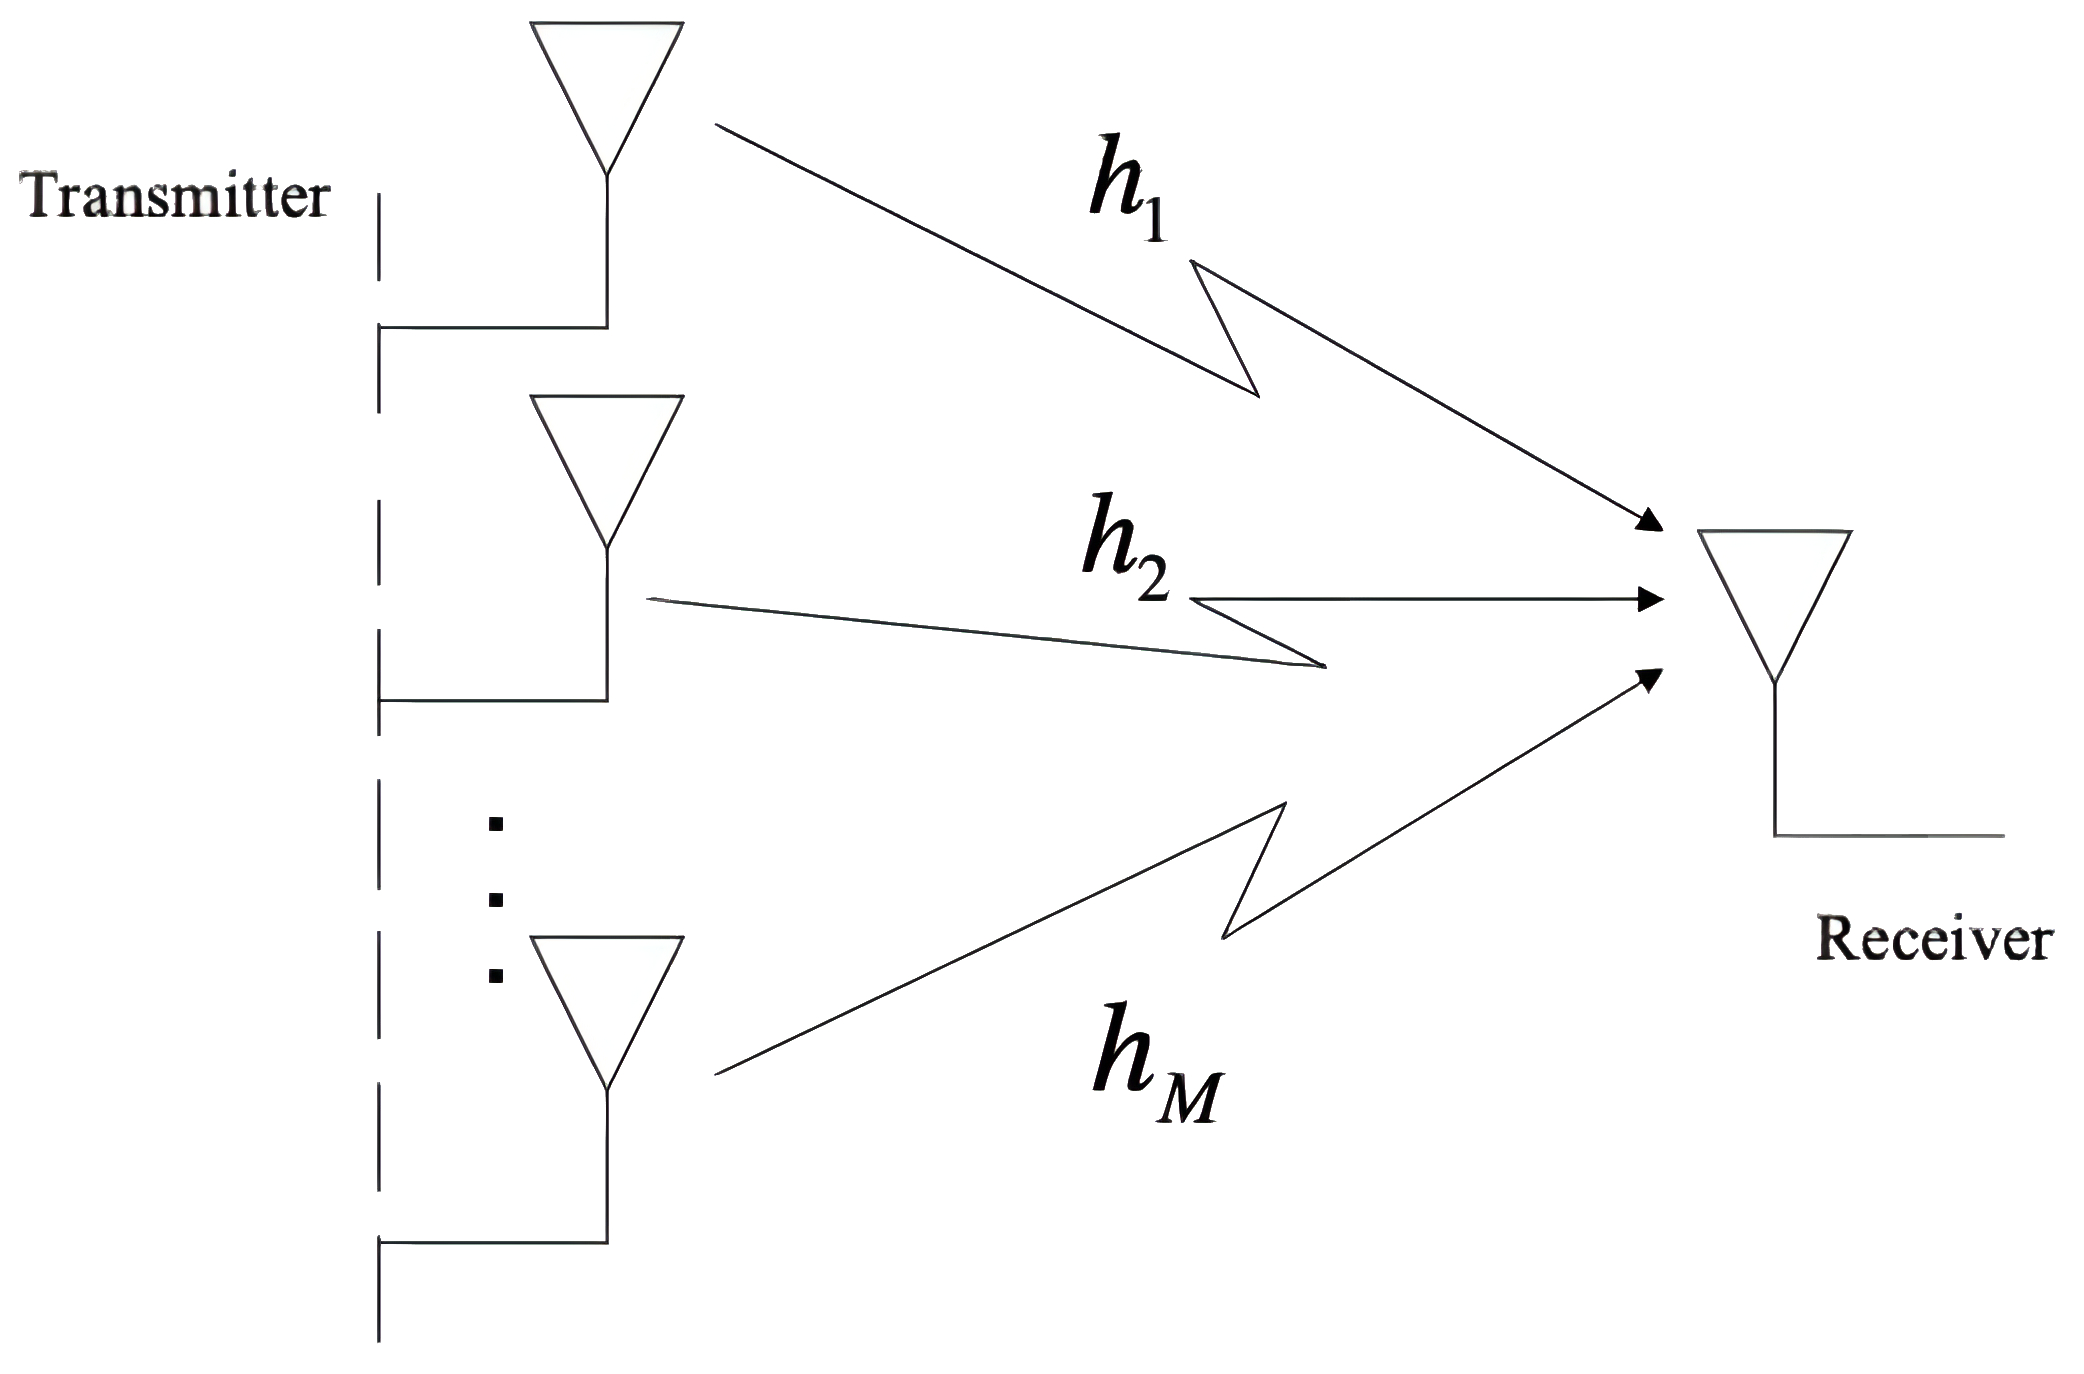
\includegraphics[width=0.4\textwidth]{imgs/miso.jpg}
\end{center}
Per quanto riguarda la configurazione con più antenne in trasmissione e singola antenna in ricezione, sistema MISO, si ottiene la stessa espressione con alcuni accorgimenti lato trasmettitore
\[
    y[m] = \mathbf{h}^T \mathbf{x}[m] + n[m] \quad \text{segnale ricevuto tramite l'unica antenna disponibile}
\]

La differenza sostanziale con il caso SIMO è che i vari segnali sono combinati ``naturalmente" durante la trasmissione e ricevuti quindi già aggregati. 
La scelta dei coefficienti non può essere effettuata lato ricevitore, ma deve essere il trasmettitore a scegliere stimando il canale, lato ricevitore la stima è ovviamente più complessa rispetto a quella che effettuerebbe il ricevitore per proprio conto.
L'operazione effettuata dal trasmettitore è detta \textbf{pre-codifica spaziale} e il simbolo è denominato \textbf{simbolo spaziale pre-codificato}.
\[
    \mathbf{x}[m] = c_m \mathbf{b} 
\]
Dove l'elemento $i$-esimo del vettore $\mathbf{x}[m]$ è il simbolo trasmesso dalla $i$-esima antenna del trasmettitore.
L'energia spesa dipende anche dal coefficiente $b_i$, l'obiettivo è comunque utilizzare la solita energia usata nel caso di singola antenna.

Il rapporto segnale/rumore (SNR) è massimizzato scegliendo $\mathbf{b} = \frac{1}{\| \mathbf{h} \|} \mathbf{h}^*$.

%\[
%    x[m] = \sum_{i=1}^{N} h_i y_i[m]  = \sum_{i=1}^{N} h_i b_i c_m + n[m] = \sum_{i=1}^{N} \frac{h_i h_i^*}{\| \mathbf{h} \|} c_m + n[m] = \| \mathbf{h} \| c_m + n[m]
%\]
\[
    y[m] = \mathbf{h}^T \mathbf{x}[m] + n[m] = c_m \mathbf{h}^T \mathbf{b} + n[m] = c_m \frac{1}{\|\mathbf{h}\|} \mathbf{h}^H \mathbf{h} + n[m] = \| \mathbf{h} \| c_m + n[m]
\]
\[
    P = \|\mathbf{h} \|^2 \ \mathbb{E} \left[\left| c_m \right|^2 \right] = \|\mathbf{h} \|^2  A
\]
\[
    P_N = \sigma^2  
\]
\[
    \text{SNR} = \frac{P}{P_N} = \frac{A}{\sigma^2} \|\mathbf{h}\|^2 
\]

La differenza tra il caso con singola antenna (sia lato trasmettitore che ricevitore) e il caso con più antenne (MISO/SIMO) è dato dal fattore $\| \mathbf{h} \| = \sum_{i=1}^{N} |h_i|^2$.
Considerando i guadagni del canale come variabili aleatorie con distribuzione di Rayleigh è possibile calcolare la distribuzione della somma come convoluzione delle PDF.
\[
    f_{\| \mathbf{h} \|^2} (x) = \frac{1}{D-1} x^{D-1} e^{-x}
\]
Il risultato dipende dal numero di antenne $D$, tuttavia in generale si ottiene un \textbf{guadagno di array}, ovvero uno spostamente del valore medio dei guadagni verso destra (più potenza).
Inoltre il \textbf{guadagno di diversità} si manifesta riducendo notevolmente la probabilità di ottenere guadagni molto bassi.
Ciò è visibile confrontando gli integrali delle due PDF.

\paragraph*{MIMO (Multiple Input Multiple Output)}

Il caso generale MIMO, ovvero con più antenne sia in trasmissione che ricezione, sfrutta una tecnica denominata \textbf{spatial multiplexing} ed è basata sulla decomposizione ai valori singolari (SVD) della matrice $\mathbf{H}$ che descrive il canale.

\paragraph*{SVD (Singular Value Decomposition)}

Data una matrice $\mathbf{A} \in \mathbb{C}^{m \times n}$, con  $p = \text{rank} (\mathbf{A})$, il SVD permette di scrivere la matrice come prodotto di tre matrici:
\[
    \mathbf{A} = \mathbf{U} \mathbf{\Sigma} \mathbf{V}^H
\]
con $\mathbf{U} \in \mathbb{C}^{m \times p}$, $\mathbf{\Sigma} \in \mathbb{C}^{p \times p}$ e $\mathbf{V} \in \mathbb{C}^{n \times p}$,
dove $\mathbf{U}$ e $\mathbf{V}$ sono matrici unitarie, mentre $\mathbf{\Sigma} = diag(\sigma_1, \ldots, \sigma_p)$ è una matrice diagonale con $\sigma_1 \geq \sigma_2 \geq \ldots \geq \sigma_p$. In un sistema MIMO, se il canale è sufficientemente multipath, la matrice $\mathbf{H}$ ha rango pieno, dunque:
\[
    p = \text{rank}(H) = \min(N_R, N_T)
\]

La tecnica di \textbf{spatial multiplexing} consiste nell'effettuare sia una pre-codifica lato trasmettitore, sia un combining lato ricevitore, dunque utilizzando due pesi differenti. In questo modo è possibile creare un certo numero di canali ortogonali indipendenti, detti \textbf{canali spaziali}.
\[
    \begin{array}{ll}
        \mathbf{H} = \mathbf{U} \mathbf{\Sigma} \mathbf{V}^H \quad \text{decomposizione SVD matrice del canale MIMO} \\
        \mathbf{B} = \mathbf{V} \quad \text{matrice pre-coder (Tx)} \\
        \mathbf{W} = \mathbf{U} \quad \text{matrice combiner (Rx)}
    \end{array}
\]
\begin{center}
    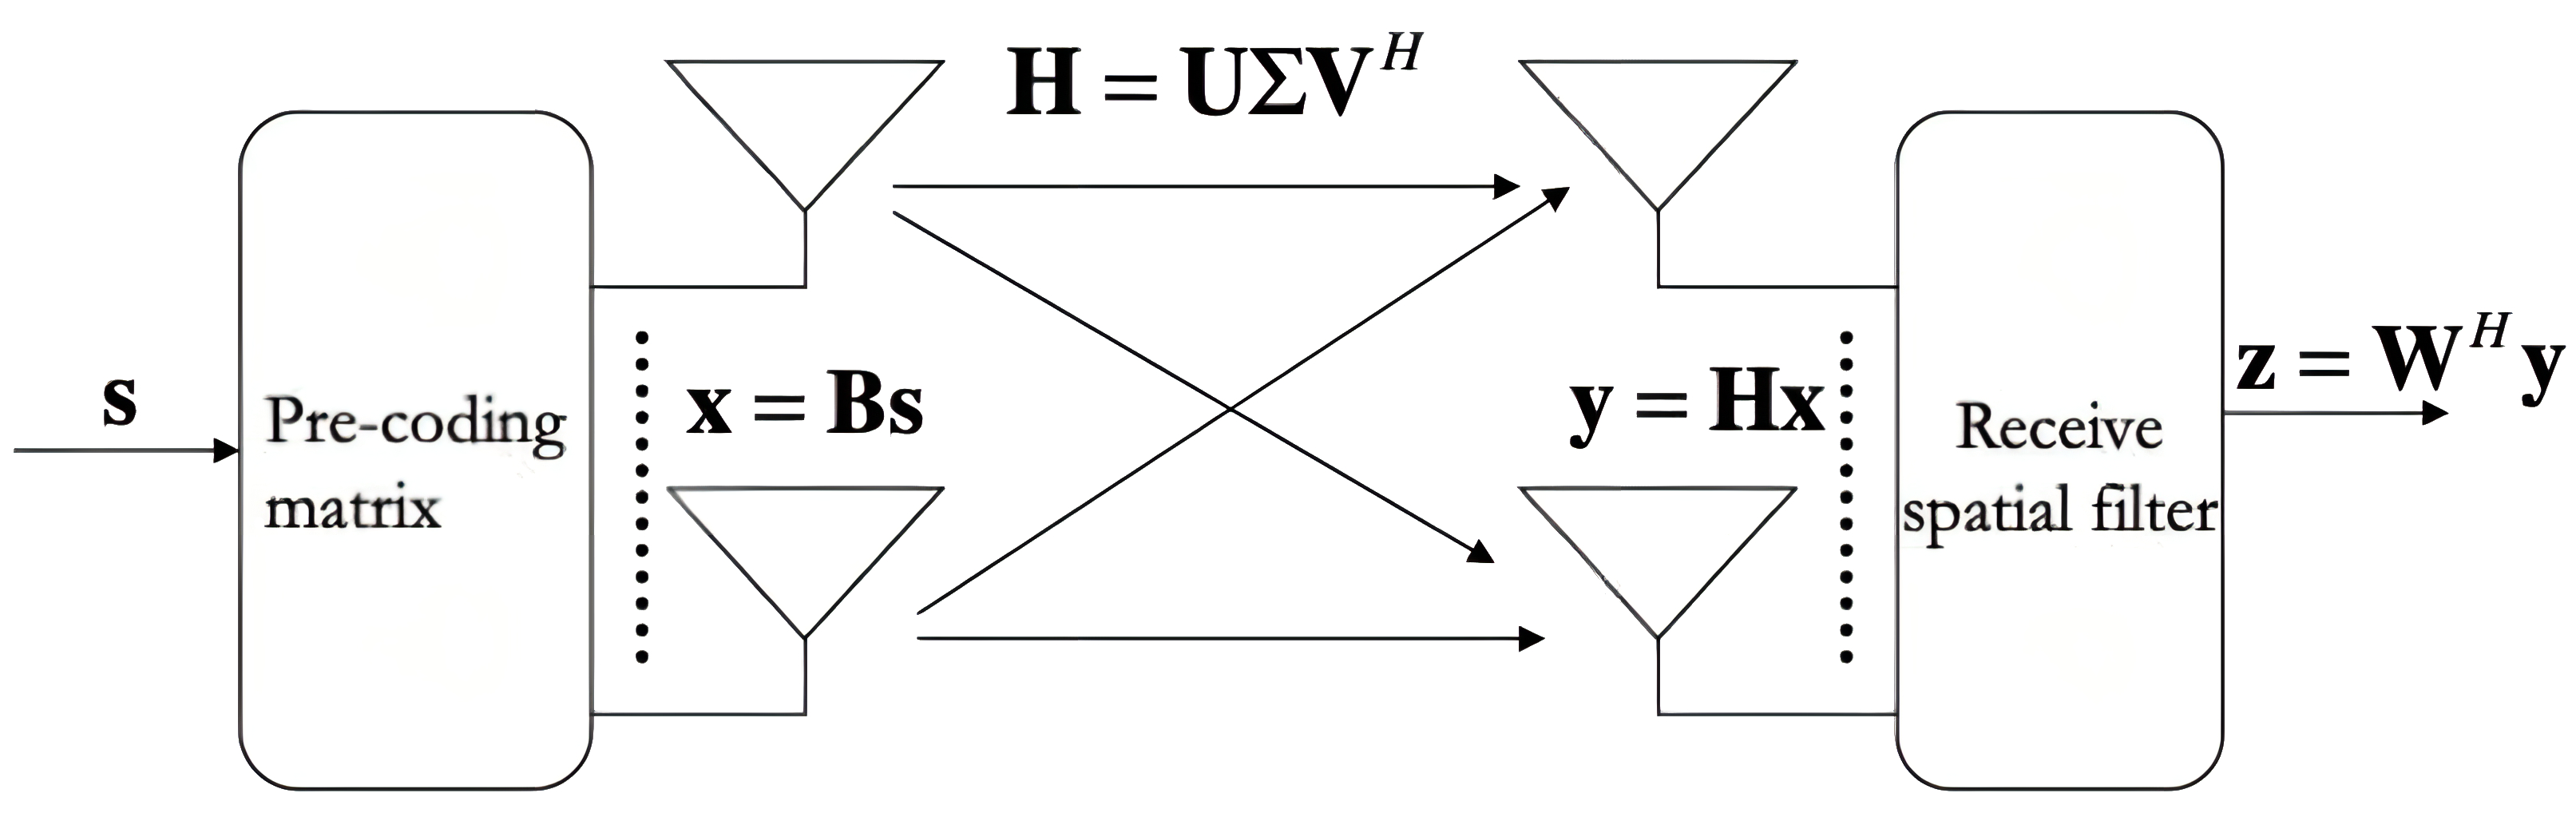
\includegraphics[width=0.8\textwidth]{imgs/mimo.jpg}
\end{center}

Scegliendo in questo modo le matrici si ottiene:
\[
    \begin{array}{ll}
        \mathbf{z} = \mathbf{W}^H \mathbf{y}  \\
        = \mathbf{W}^H \left( \mathbf{H} \mathbf{x} + \mathbf{n}  \right) \\  
        = \mathbf{W}^H \left( \mathbf{H} \mathbf{B} \mathbf{s} + \mathbf{n} \right) \\
        = \mathbf{W}^H \mathbf{H} \mathbf{B} \mathbf{s} + \mathbf{W}^H \mathbf{n}  \\
        = \mathbf{U}^H \mathbf{H} \mathbf{V} \mathbf{s} + \mathbf{W}^H \mathbf{n} \\
        = \mathbf{\Sigma} \mathbf{s} + \mathbf{W}^H \mathbf{n}
    \end{array}
\]
Sebbene ogni antenna riceva dei segnali sovrapposti, scegliendo le matrici in questa maniera è possibile ottenere dei canali ortogonali che non interferiscono tra loro dato che la matrice $\mathbf{\Sigma}$ è diagonale.
Quindi $\mathbf{s}$ è trasmesso su $p = rank(\mathbf{H})$ canali indipendenti.
Dato che il rango della matrice del canale è maggiore di 1, la capacità del canale è incrementata di un fattore pari al rango della matrice del canale. Questo non è possibile in sistemi SIMO o MISO, in cui il rango è pari a 1.

Considerando un sistema $2 \times 2$ per esempio si ottiene:
\[
    \begin{cases*}
        y_1 = h_{11} x_1 + h_{12} x_2 + n_1 \\
        y_2 = h_{21} x_1 + h_{22} x_2 + n_2
    \end{cases*}
    \quad
    \text{segnali sovrapposti su ogni antenna}
\]

L'utilizzo di un canale MIMO può incrementare la capacità del sistema, tuttavia è necessario tenere in considerazione anche i valori singolari, i quali potrebbero comportare un'attenuazione eccessiva.


\[
    \mathbf{z} = \begin{matrix}
        \begin{bmatrix}
            \sigma_1 s_1 + n_1' \\
            \sigma_2 s_2 + n_2'
        \end{bmatrix}
    \end{matrix}
    \quad 
    \text{segnale ottenuto dopo combining lato ricevitore, non c'è alcuna sovrapposizione}
\]

\section*{Diversità in frequenza}

La formula di Shannon fornisce il massimo rate sostenibile su un dato canale di trasmissione:
\[
    C = B \log_2 \left( 1 + \text{SNR} \right), \quad \text{SNR} = \frac{\left| H \right|^2 P}{\sigma^2}
\]
Dove $H$ è il guadagno del canale.
In sistemi reali ci si può solo avvicinare al limite teorico e vi è una forte dipendenza, per quanto riguarda l'efficienza spettrale, del coding rate e modulation order, data dalla dimensione della costellazione di simboli per cui esiste un trade-off tra capacità di trasmissione ed energia richiesta.
In particolare $\log_2 \left( 1 + \text{SNR} \right)$ è l'efficienza spettrale.
Il rate di trasmissione reale può essere approssimato:
\[
    R_b = \log_2 M \  R \frac{1}{T}  \approx m R B
\]

Dove è $M$ è il numeri di simboli nella costenllazione, $R$ è il coding rate \footnote{con $R_s$ indichiamo il symbol rate, ovvero $\frac{1}{T}$, mentre con $R$ il coding symbol rate} e $T$ è il symbol time, si fa l'approssimazione che $\frac{1}{T} \approx B$. 


Per rispettare il limite di capacità si deve avere:
\[
    m R B < C \quad \Rightarrow \quad m R < \log_2 (1 + \text{SNR})
\]
Misurando il SNR è possibile adattare i valori di $m$ ed $R$, ad esempio in base alla posizone in una cella.
I valori di $m$ ed $R$ che si possono utilizzare appartengono ad un insieme finito, non è possibile scegliere arbitrariamente.

\begin{table}[H]
    \resizebox{\textwidth}{!}{
        \centering
        \begin{tabular}{|c|l|c|c|c|}
        \hline
        \textbf{Radio Bearer Index} & \textbf{Name} & \textbf{Modulation} & \textbf{Channel Coding Rate} & \textbf{Bearer Efficiency} ($\log_2(1+\text{SNR})$, bits/symbol) \\ \hline
            1  & QPSK 1/12 & QPSK & 0.0761719 & 0.1523 \\ \hline
            2  & QPSK 1/9  & QPSK & 0.117188  & 0.2344 \\ \hline
            3  & QPSK 1/6  & QPSK & 0.188477  & 0.377  \\ \hline
            4  & QPSK 1/3  & QPSK & 0.300781  & 0.6016 \\ \hline
            5  & QPSK 1/2  & QPSK & 0.438477  & 0.877  \\ \hline
            6  & QPSK 3/5  & QPSK & 0.587891  & 1.1758 \\ \hline
            7  & 16QAM 1/3 & 16QAM & 0.369141  & 1.4766 \\ \hline
            8  & 16QAM 1/2 & 16QAM & 0.478516  & 1.9141 \\ \hline
            9  & 16QAM 3/5 & 16QAM & 0.601563  & 2.4063 \\ \hline
            10 & 64QAM 1/2 & 64QAM & 0.455078  & 2.7305 \\ \hline
            11 & 64QAM 1/2 & 64QAM & 0.553711  & 3.3223 \\ \hline
            12 & 64QAM 3/5 & 64QAM & 0.650391  & 3.9023 \\ \hline
            13 & 64QAM 3/4 & 64QAM & 0.753906  & 4.5234 \\ \hline
            14 & 64QAM 5/6 & 64QAM & 0.852539  & 5.1152 \\ \hline
            15 & 64QAM 11/12 & 64QAM & 0.925781  & 5.5547 \\ \hline
        \end{tabular}
    }
\end{table}

Come si evince dalla tabella, in pratica c'è un mapping diretto tra SNR misurato (channel quality indicator, CQI) e lo specifico ordine di modulazione e coding rate di una trasmissione.
La qualità del canale in termini di SNR può essere espressa tramite \textbf{radio beared index} ($\in [1, 15]$).
Utilizzando la modulazione OFDM l'idea sarebbe adattare $m$ ed $R$ per ogni canale, distribuendo la potenza nel modo più efficace possibile per massimizzare il rate di trasmissione. Questo problema è indicato con il termine di \textbf{water-filling}, la potenza a disposizione è invece detta \textbf{power budget}. Nella pratica si tratta di un problema di ottimizzazione per il quale sono definiti alcuni vincoli da rispettare:

% TODO: p non lo metterei, perché non è chiaro cosa rappresenti
\[
    \begin{cases}
       \underset{\mathbf{p}}{\text{max}} \sum_{n=1}^{N} \log_2(1 + \frac{P_n}{\sigma_n^2}) \\
       \sum_{n=1}^{N} P_n = P_0 \quad \text{(power budget)} \\
        P_n \geq 0 \quad n = 1, \ldots, N
    \end{cases}    
\]

Dove $\sigma_n^2 = \frac{\sigma^2}{\left| \mathbf{H}_{n, n} \right| ^2}$. Il termine $B$ non appare nell'espressione in quanto costante per ogni canale, massimizzare il rate o l'efficienza spettrale genera lo stesso risultato.

La lagrangiana del problema è:
\[
    \mathcal{L}(P_1, \hdots, P_N, \lambda ) = \sum_{n=1}^{N} \log_2(1 + \frac{P_n}{\sigma_n^2}) - \lambda \left( \sum_{n=1}^{N} P_n - P_0 \right)
\]
La derivata rispetto a $P_k$ posta a 0 per la condizione di stazionarietà è:
\[
    \frac{\partial \mathcal{L}}{\partial P_k} = \frac{1}{\ln(2)} \frac{1}{\sigma_k^2 + P_k} - \lambda = 0, \quad k = 1, \ldots, N
\]
ovvero il gradiente:
\[
    \nabla_{P_1, \hdots, P_N} \mathcal{L} = \begin{bmatrix}
        \frac{1}{\ln(2)} \frac{1}{\sigma_1^2 + P_1} - \lambda \\
        \frac{1}{\ln(2)} \frac{1}{\sigma_2^2 + P_2} - \lambda \\
        \vdots \\
        \frac{1}{\ln(2)} \frac{1}{\sigma_N^2 + P_N} - \lambda
\end{bmatrix} = \mathbf{0}
\]
La soluzione del problema è:
\[
    \hat{P}_n = \frac{1}{\lambda \ln(2)} - \sigma_n^2, \quad n = 1, \ldots, N
\]
considerando il vincolo che $P_n \geq 0$ e ponendo $\mu = \frac{1}{\lambda \ln(2)}$ si ottiene:
\[
    \hat{P}_n = \text{max} \{ 0, \mu - \sigma_n^2    \} = (\mu - \sigma_n^2)^+, \quad n = 1, \ldots, N
\]
Per ottenere dei valori è necessario calcolare $\mu$, scelto in modo da rispettare il vincolo sulla potenza a disposizione.
\[
    \sum_{n=1}^{N} (\mu - \sigma_n^2)^+ = P_0
\]
\[
    \begin{cases}
        f(\mu) = \sum_{n=1}^{N} (\mu - \sigma_n^2)^+ - P_0 \\
        f: \mathbb{R}^n \rightarrow \mathbb{R}
    \end{cases}
\]
La risoluzione dell'equazione garantisce il valore $\mu$ tale per cui i vincoli sono rispettati, è quindi necessario trovare lo zero di una funzione in $\mu$, ad esempio con il metodo di bisezione, che può essere applicato dato che la funzione risulta continua e monotona su
Il termine water-filling deriva dal fatto che osservando il grafico della distribuzione della potenza, si ha l'impressione che la potenza si distribuisca come l'acqua all'interno di un contenitore con superficie irregolare, fino ad un livello pari a $\mu$.
La distribuzione è ottima e rappresenta la miglior situazione per sfruttare la diversità in frequenza del canale.
In sostanza la distribuzione favorisce i canali con miglior qualità, scartando completamente quelli la cui capacità è troppo bassa, quindi la maggior parte della potenza verrà allocata alle frequenze con le migliori condizioni di canale e più alto SNR.

